%%
%% (
%%  )\ )                             (
%%  (()/(   (            (             )\  )   (
%%   /(_))  ))\   (       ))\  (   (   (()/(   ))\
%%   (_))  /((_)  )\  )  /((_) )\  )\   ((_))/((_)
%%   | _ \(_))(  _(_/( (_) )  ((_)((_)  _| |(_))
%%   |   /| || || ' \))/ -_)/ _|/ _ \/ _` |/ -_)
%%   |_|_\ \_,_||_||_| \___|\__|\___/\__,_|\___|
%%

\documentclass{article}
\usepackage[utf8x]{inputenc}
\usepackage{amsmath}
%\usepackage{slashbox}
\usepackage{amsfonts}
\usepackage{amssymb}
\usepackage{graphicx} % Paquete para incluir imágenes en el documento LaTeX
\usepackage{hyperref}
\hypersetup{
  colorlinks=true,
  linkcolor=blue,
  filecolor=magenta,
  urlcolor=cyan,
}
\urlstyle{same}
\usepackage{varwidth}

\newcommand\tab[1][1cm]{\hspace*{#1}}

\usepackage{multirow}

\usepackage[a4paper,rmargin=1.5cm,lmargin=1.5cm,top=1.5cm,bottom=1.5cm]{geometry}

\usepackage{pdfpages}

\usepackage{xcolor}
\usepackage{minted}
\setminted[mysql]{frame=lines, framesep=2mm, baselinestretch=1.2, rulecolor=\color{black!80}, bgcolor=DarkGray}
\usemintedstyle[mysql]{monokai}
\setminted[python3]{frame=lines, framesep=2mm, baselinestretch=1.2, rulecolor=\color{black!80}, bgcolor=DarkGray}
\usemintedstyle[python]{paraiso-dark}
\setminted[./pseudocode.py:PseudocodeLexer -x]{frame=lines, framesep=2mm, baselinestretch=1.2,
            rulecolor=\color{black!30}, bgcolor=LightGray}
\usemintedstyle[./pseudocode.py:PseudocodeLexer -x]{rainbow_dash}
\setminted[bash]{baselinestretch=1.2,rulecolor=\color{black!30},fontsize=\footnotesize,bgcolor=LightGray}
\definecolor{LightGray}{gray}{0.98}
\definecolor{DarkGray}{gray}{0.1}
\definecolor{MidGray}{gray}{0.8}
\definecolor{codegreen}{rgb}{0,0.6,0}
\definecolor{codegray}{rgb}{0.5,0.5,0.5}
\definecolor{codepurple}{rgb}{0.58,0,0.82}
\definecolor{backcolour}{rgb}{0.95,0.95,0.92}

\setlength{\parindent}{0px}  % Setea la indentacion de la primera linea de cada parrafo a cero pixeles.


\title{Resolución de la novena semana}
\author{@RuneCode}

\begin{document}
%% Portada
\includepdf{./portada/portada.pdf}

%% Clase 1
\section{Bienvenida conceptos básicos y contexto histórico de las Bases de Datos}%

\textbf{Historia de Base de datos}

Desde la antiguedad se quería tener persistencia de la información y para esto
se desarrollaron sistemas de escritura en piedra o arcilla, luego el papiro que
permitía mayor portabilidad de los documentos pero no eran tan resistentes ya
que se descomponían o eran anidados por hongos y finalmente los chinos que
inventaron el papel que tenía las ventajas de ser fáciles de transportar pero
también muy resistentes.

Pasaron muchos siglos y el siguiente salto que se logró después del papel se
dio en el siglo XX con el microfilm que tiene la ventaja de almacenar
información que puede durar miles de años sin ningún problema, la desventaja es
que el guardar, modificar y leer información requiere de máquinas muy
especializadas que no son fáciles de conseguir y no es tan fácil el proceso
tampoco.\\

Luego tenemos a los medios digitales: Los discos duros, discos de estado
sólido, incluso los CDs fueron medios de almacenamiento digital en los que para
su almacenamiento se usó el formato digital de "unos y ceros".

El siguiente gran cambio que se dió fue la nube. La nube tiene como beneficio a
su favor el que es accesible desde cualquier parte del mundo.

Entonces \textbf{¿Qué son las Bases de Datos?}
Las bases de datos entran en el periodo en el que hicimos la transición a
medios digitales y ahora en la nube.
Las bases de datos nos servian para complementar la arquitectura de Von Neumann
(que es la arquitectura de computación clásica que contiene un CPU, memoria y
elementos de entrada y salida).

Las bases de datos se han divido en dos grandes tipos, las Relacionales, que
fueron las primeras en surgir y luego las no relacionales.\\

Con respecto a las \textbf{Bases de Datos relacionales} actualmente tenemos en
la industria varias compañías que se dedican a ser manejadores de Base de Datos
Relacionales, por ejemplo SQL Server de Microsoft, luego Oracle que ha sido muy
popular e importante; pero tenemos también las versiones de comunidad u Open
Source, por ejemplo PostgresSQl, la más usada probablemente en la industria que
es MySQL que aunque ahora pertenece a Oracle anteriormente era de Sun
Microsistem y como respuesta a esta adquisición de MySQL también se crea
MariaDB que es virtualmente lo mismo que MySQL de hecho es un fork del codigo
original que hizo su creador para continuar con este proyecto de una manera más
libre sin tener que estar atado a Oracle.

Con respecto a las \textbf{Bases de Datos no Relacionales} es un mundo muy
interesante y que todavía está avanzando por ejemplo: MemcacheDB, Cassandra que
es una base datos que inventó Facebook, DynamoDB, elasticsearch, BigQuery, y
también tenemos algunas muy interesantes como: neo4j (basada en grafos),
MongoDB (una de las más utilizadas) y tenemos firestore que es una muy
reciente.

Tenemos también otra gran división de servicios de Base de Datos: Los que se
llaman \textbf{Autoadministrados y los Administrados}. Los Autoadministrados,
es la base de datos que tu instalas en tu computadora o en tu servidor, tu te
encargas de las actualizaciones y te encargas de toda la parte de
mantenimiento, actualización, parche, persistencia de datos, etc. Los servicios
administrados por otro lado no se manejan por uno mismo, son servicios que
ofrecen las nubes modernas, por ejemplo: Amazon, Google o Azure de Microsoft
que lo que te ofrecen es realmente el servicio de base de datos. Tu vas a
usarla pero no tienes que instalarla u ocuparte de todo el mantenimiento que
implica. Como se ve ambas tienen ciertas ventajas y desventajas.

%% clase 2
\section{Historia de las RDB}%
Las bases de datos surgen de la necesidad de conservar la información más allá
de lo que existe en la memoria RAM (en el esquema de la arquitectura de Von
Neumann). Y cuando tuvimos la necesidad de guardar la información de una forma
que fuera facil de guardar y extraer empezaron a buscarse formas un poquito más
inteligentes de hacerse esto. La primera aproximación fueron lo que se llaman
Base de Datos basados en archivos que no es lo mismo que Base de Datos basados
en Documentos.\\

Las bases de datos basadas en archivos eran datos guardados en texto plano,
fáciles de guardar pero muy difíciles de consultar y por la necesidad de
mejorar nacen las \textbf{bases de datos relacionales}. Su inventor
\textbf{Edgar Codd} dejó ciertas reglas para asegurarse de que toda la
filosofía de las bases de datos no se perdieran, estandarizando el proceso.
(Codd inventó algo llamado el Álgebra Relacional.)\\

%% Clase 3
\section{Entidades y atributos}%
Una \textbf{entidad} es algo similar a un objeto (programación orientada a
objetos) y representa algo en el mundo real, incluso algo abstracto. Las
entidades tienen atributos que son las características que las hacen ser una
entidad y por convención se ponen en plural.

\newpage
Veamos unos diagramas de ejemplo:
\begin{figure}[h!]
    \centering
      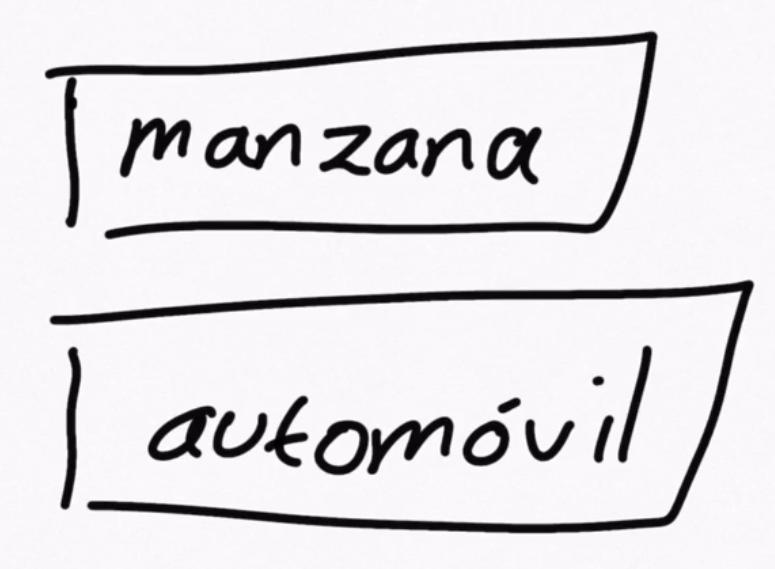
\includegraphics[scale=0.5]{./Pictures/001_entidades.png}
\end{figure}

\begin{figure}[h!]
    \centering
      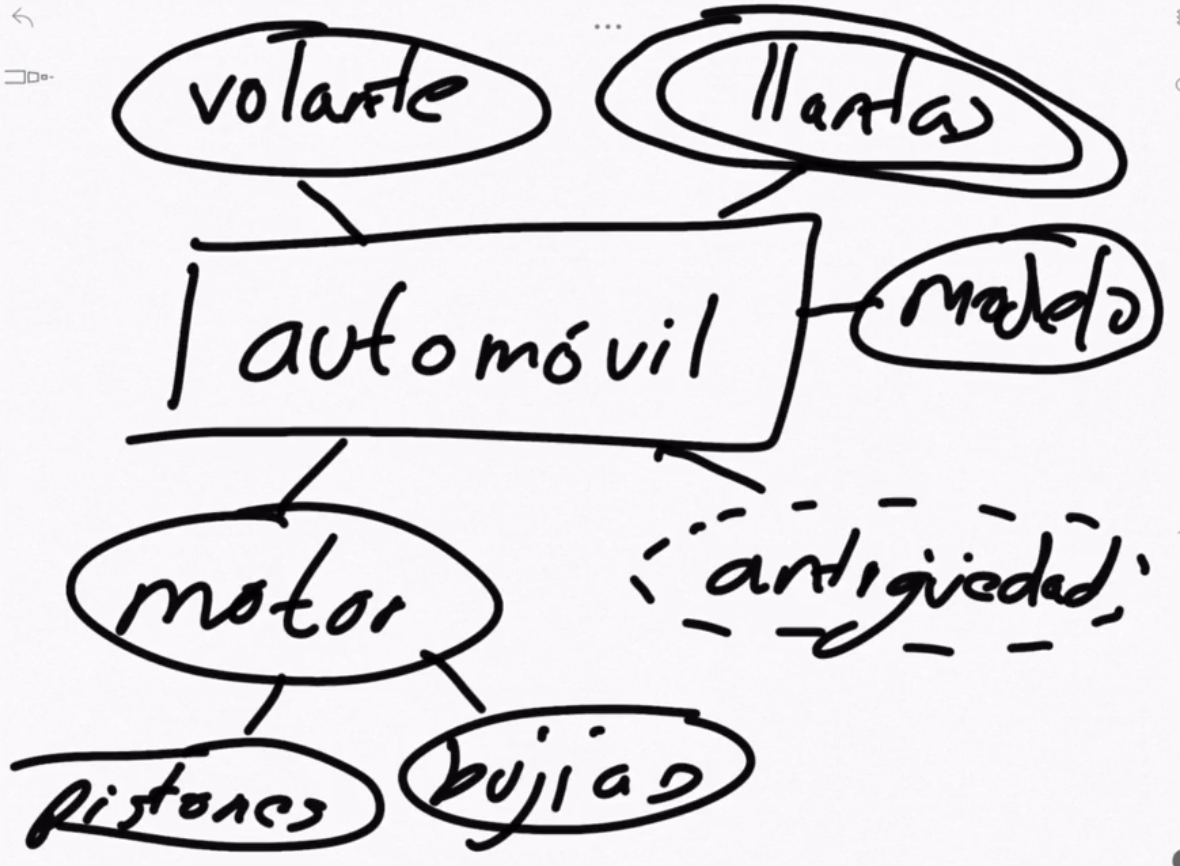
\includegraphics[scale=0.5]{./Pictures/002_Diagrama.png}
\end{figure}

El atributo \textbf{llantas} es un \textbf{atributo multivaluado}, eso quiere
decir que la entidad \textbf{automóvil} tiene más de uno de estos atributos.
Como se vé, se representa con un \textbf{ovalo doble}.\\

Ahora veamos el atributo \textbf{motor} es un \textbf{atributo compuesto} ya
que, este a su vez está formado por otros atributos.\\

También fijémonos en el \textbf{atributo especial} llamado \textbf{antiguedad},
ya que este atributo se puede inferir a partir del año en el que salió el
automovila. Se representa con un óvalo discontinuo.

\newpage

\begin{figure}[h!]
    \centering
      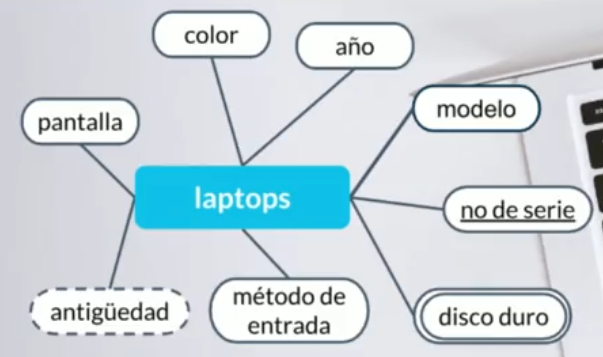
\includegraphics[scale=0.5]{./Pictures/003_atributos.png}
\end{figure}

Por convención las entidades se ponen en plural.\\

En caso del atributo \textbf{no\_de\_serie} es el que diferencia nuestra
entidad de otras y se conoce como atributo llave, se grafica dentro de un óvalo
y además tiene subrayado.

\begin{figure}[h!]
    \centering
      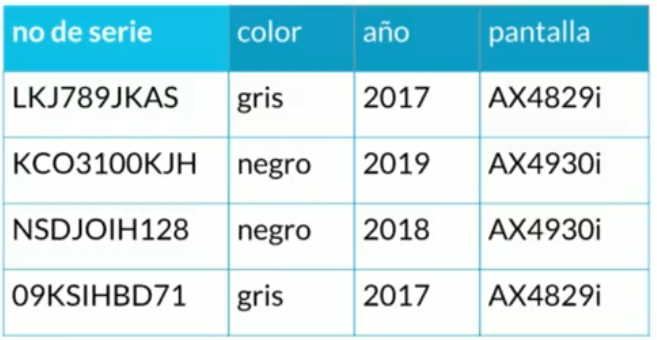
\includegraphics[scale=0.5]{./Pictures/004_id.png}
\end{figure}

Los \textbf{atributos compuestos} son aquellos que tienen atributos ellos
mismos.

Los \textbf{atributos llave} son aquellos que identifican a la entidad y no
pueden ser repetidos. Existen:

\begin{itemize}
  \item Naturales: Son inherentes al objeto como el número de serie.
  \item Clave artificial: No es inherente al objeto y se asigna de manera arbritaria.
\end{itemize}

\textbf{Entidades débiles}: No pueden existir sin una entidad fuerte y se representan
con un cuadrado con doble línea.

\begin{figure}[h!]
    \centering
      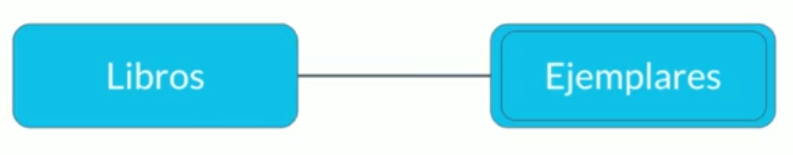
\includegraphics[scale=0.5]{./Pictures/005_entidades_debiles.png}
\end{figure}

La Identidades pueden ser débiles por dos motivos:\\

\textbf{Entidades débiles por idendidad:} No se diferencian entre si más que
por la clave de su entidad fuerte.

\begin{figure}[h!]
    \centering
      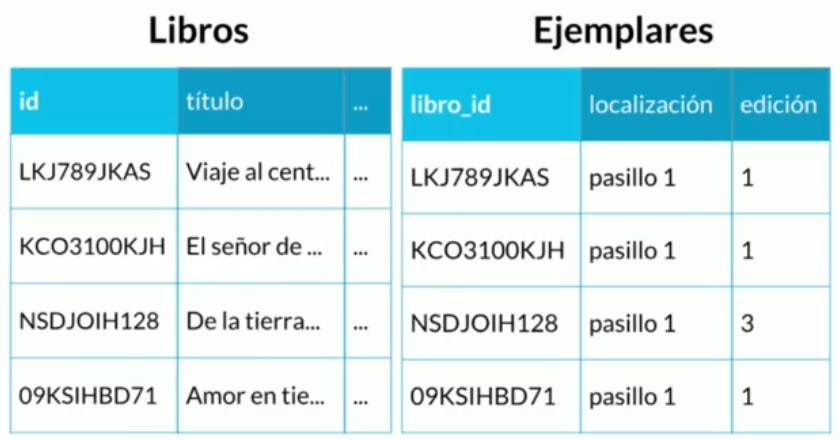
\includegraphics[scale=0.5]{./Pictures/006_entidades_debiles_dependientes.png}
\end{figure}

\newpage
\textbf{Entidades débiles por existencia}: Se les asigna una clave propia,
pero conceptualmente no puede existir esta identidad sin otra que sea fuerte.

\begin{figure}[h!]
    \centering
      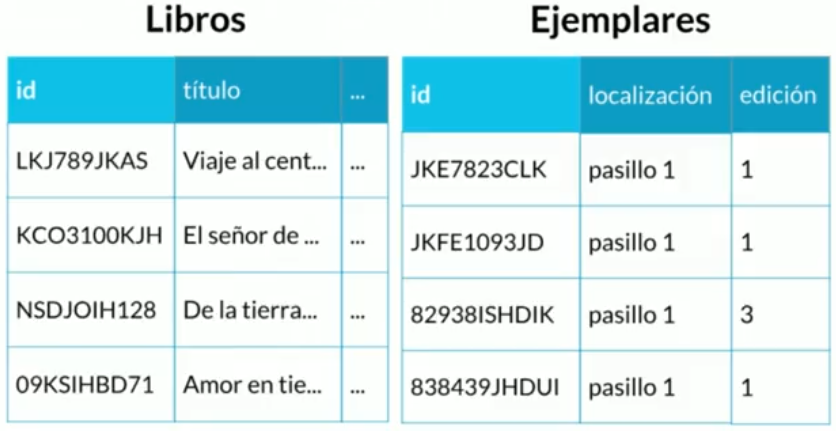
\includegraphics[scale=0.5]{./Pictures/007_enditad_debil_existencia.png}
\end{figure}


%% Clase 4
\section{Entidades de Platzi Blog}%
Nuestro proyecto será un manejador de Blogpost. Es un contexto familiar y nos
representará retos muy interesantes.\\

Primer paso: Identificar las entidades.\\
Segundo paso: Pensar en los atributos.\\

Diagrama ER (Entidad - Relación): Platziblog\\

Veamos las entidades
\begin{figure}[h!]
    \centering
      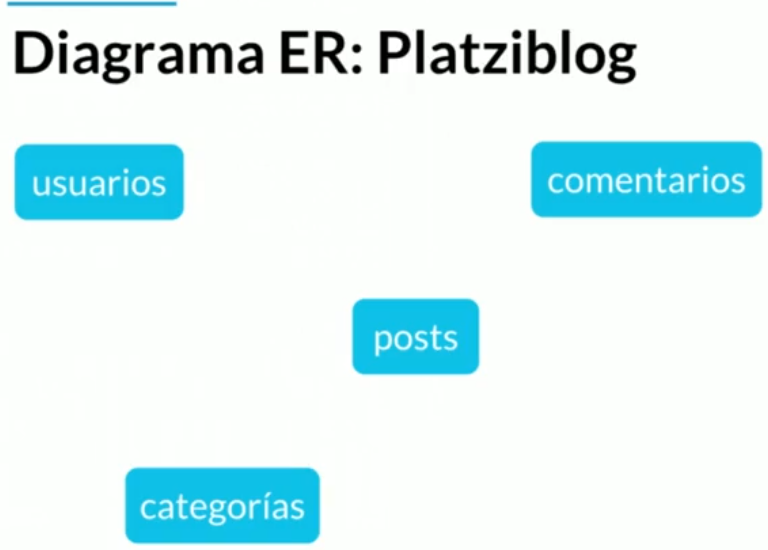
\includegraphics[scale=0.45]{./Pictures/008_Diagrama.png}
\end{figure}

Ahora los atributos de cada Entidad:

\begin{figure}[h!]
    \centering
      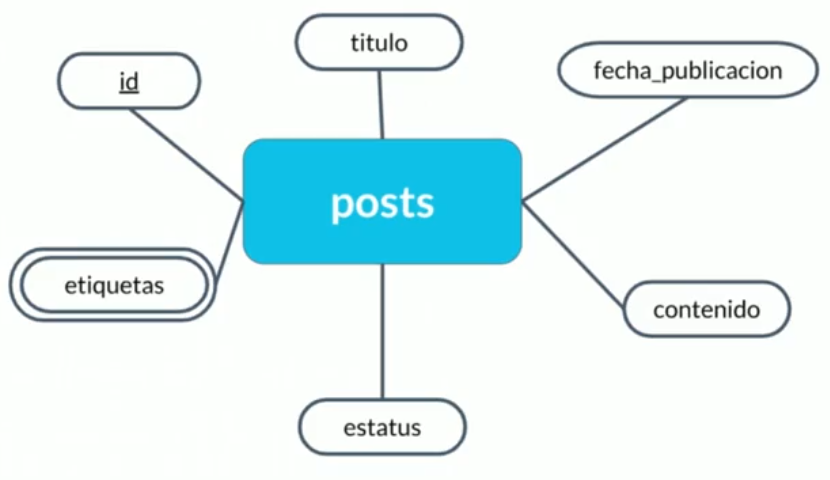
\includegraphics[scale=0.45]{./Pictures/009_post.png}
\end{figure}

\begin{figure}[h!]
    \centering
      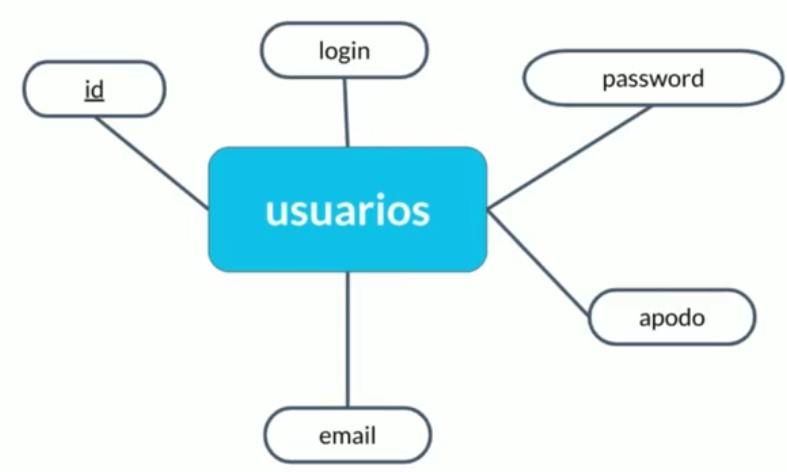
\includegraphics[scale=0.45]{./Pictures/010_usuarios.png}
\end{figure}


%% Clase 5
\section{Relaciones}%
Las \textbf{relaciones} nos permiten ligar o unir nuestras diferentes entidades
y se representan con rombos. Por convención se definen a través de verbos.\\

Por ejemplo veamos dos entidades, \textbf{Automóvil} y \textbf{Dueño} que son
entidades que se van a vincular con la relación lamado \textbf{tiene}.\\

\begin{figure}[h!]
    \centering
      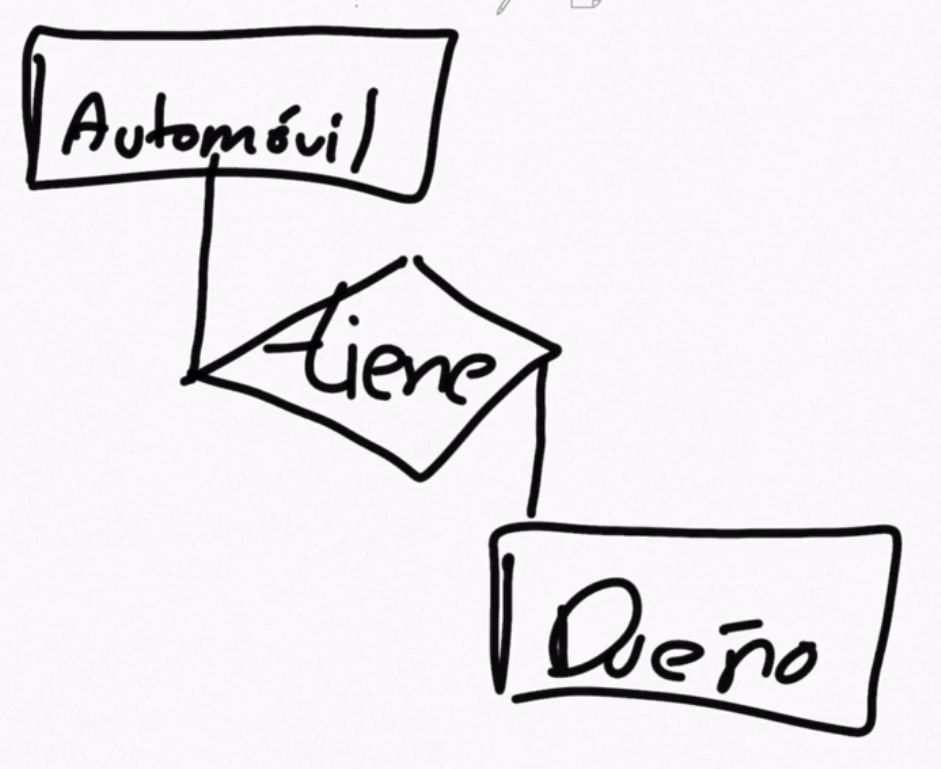
\includegraphics[scale=0.35]{./Pictures/011_relacion_tiene.png}
\end{figure}

Ahora veamos por ejemplo las entidades \textbf{Jugadores} y \textbf{Equipos}
que vamos a vincular con la relación llamado \textbf{pertenece}.

\begin{figure}[h!]
    \centering
      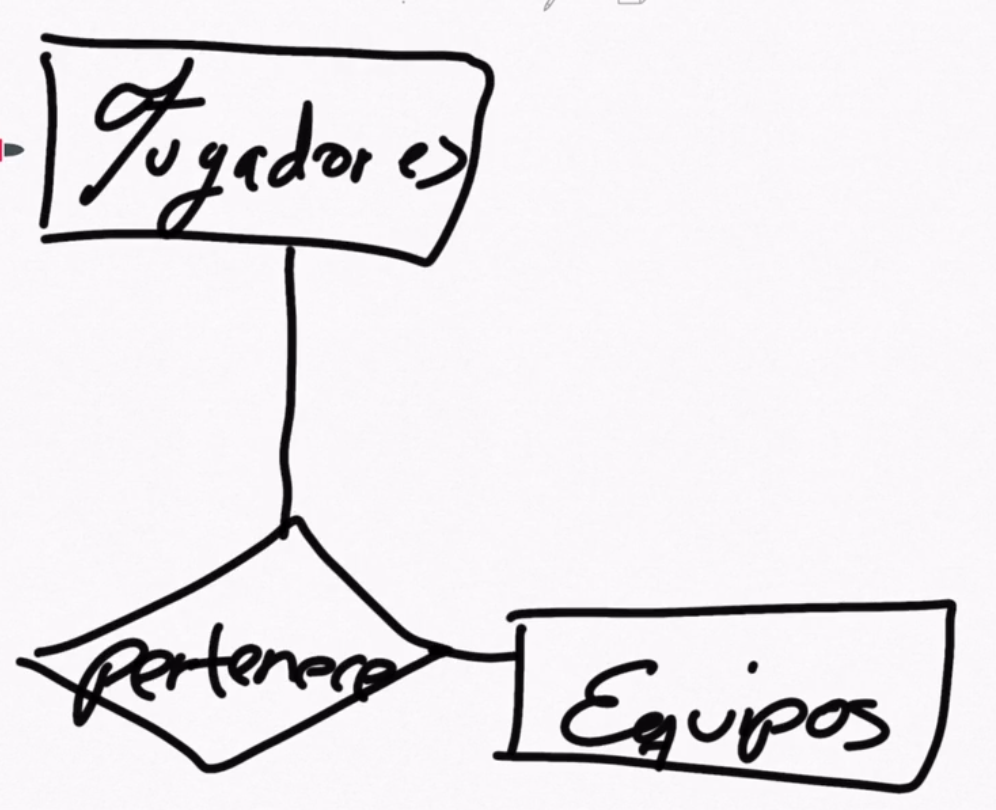
\includegraphics[scale=0.35]{./Pictures/011_relacion_pertenece.png}
\end{figure}

También veamos otras dos entidades: \textbf{laptops} y \textbf{discos\_duros}
(este último era un atributo multivaluado), cuando tenemos \textbf{atributos
multivaluados} por lo general los convertimos en entidades separadas porque
tienen una vida en sí mismas. En este caso decimos que una laptop tiene varios
discos\_duros y esto se define con la cardinalidad.\\

\begin{figure}[h!]
    \centering
      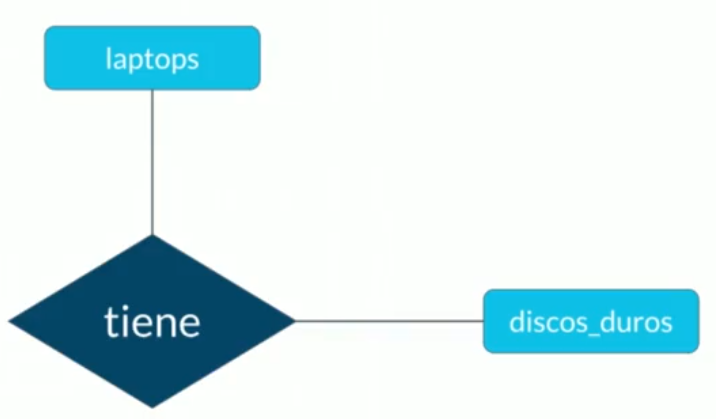
\includegraphics[scale=0.40]{./Pictures/012_relacion_tiene.png}
\end{figure}

Las relaciones tienen una propiedad llamada \textbf{cardinalidad} y tiene que
ver con números. Cuántos de un lado pertenecen a cuántos del otro lado:

\begin{itemize}
  \item Cardinalidad: 1 a 1
  \item Cardinalidad: 0 a 1
  \item Cardinalidad: 1 a N
  \item Cardinalidad: 0 a N
\end{itemize}

\textbf{Cardinalidad: 1 a 1}\\
Por ejemplo veamos la cardinalidad de una entidad \textbf{persona} con
\textbf{datos\_contacto}. Vamos hacer el enunciado de 1 \textbf{persona}
cuántos \textbf{datos\_contacto} tiene y esa relación es de 1 a 1. De igual
manera analizamos pero en sentido contrario, 1 \textbf{datos\_contacto}
pertenecen a 1 \textbf{persona}. Para obtener la cardinalidad se verifica el
mayor número de ambos lados. Que en este caso es 1 a 1.

\begin{figure}[h!]
    \centering
      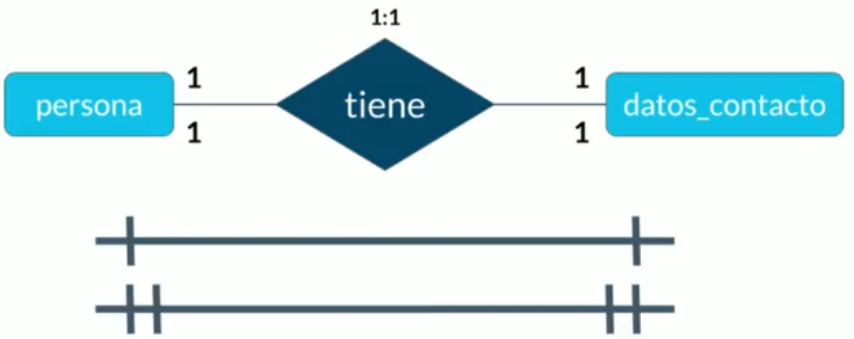
\includegraphics[scale=0.45]{./Pictures/014_card_1_1.png}
\end{figure}

Este diagrama es llamado de \textbf{Entidad Relación}. Esta relación también se
puede representar con el conector que se ve en el grafico, que es llamado
diagrama físico de base de Datos.\\

\textbf{Cardinalidad: 0 a 1}\\
Esta cardinalidad es opcional, por ejemplo puede que haya una
\textbf{sesion\_actual} para un usuario como tambien que no.

\begin{figure}[h!]
    \centering
      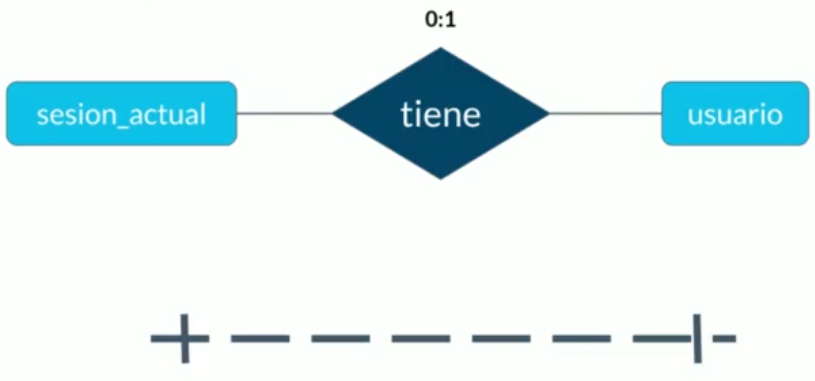
\includegraphics[scale=0.45]{./Pictures/015_card_0_1.png}
\end{figure}

\newpage

\textbf{Cardinalidad: 1 a N}\\
Esta es la cardinalidad 1 a muchos, por ejemplo: Una persona afortunada, puede
tener muchos automóviles, sin embargo un automóvil por tema de papeles y demás
solo puede pertenecer a una persona. De igual forma, para obtener la
cardinalidad se saca el número mayor de cada lado.\\

\begin{figure}[h!]
    \centering
      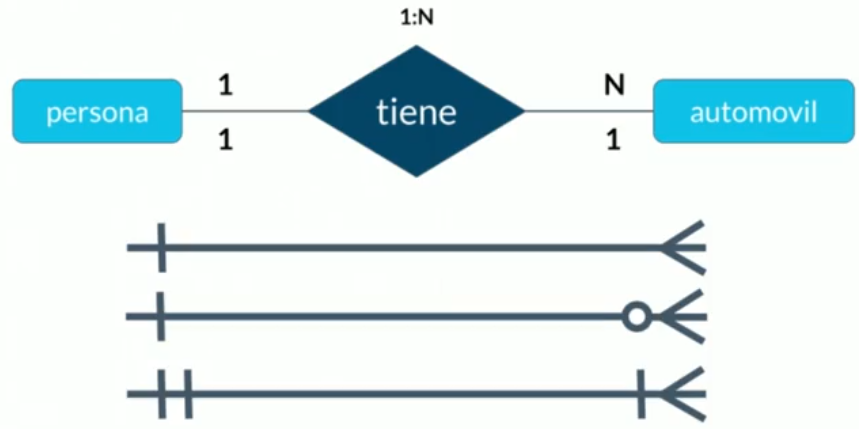
\includegraphics[scale=0.45]{./Pictures/016_card_1_N.png}
\end{figure}

\textbf{Cardinalidad: 0 a N}\\
Por ejemplo en el siguiente esquema podemos observar que una hab\_hospital
puede tener muchos pacientes, pero también puede estar vacía, es decir es
opcional.

\begin{figure}[h!]
    \centering
      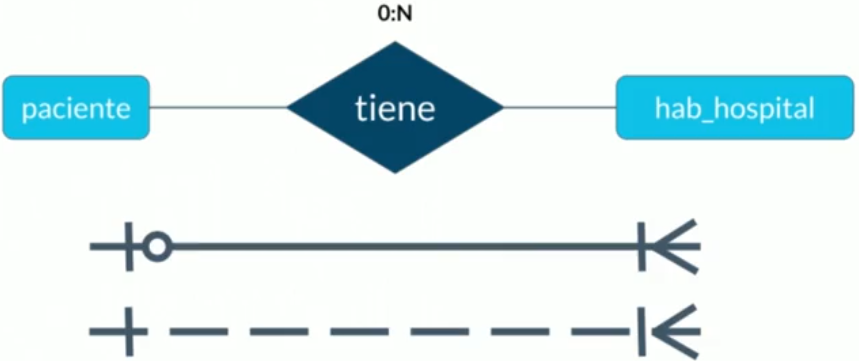
\includegraphics[scale=0.45]{./Pictures/017_card_0_N.png}
\end{figure}


%% Clase 6
\section{Multiples muchos}%
Es un tipo de cardinalidad muy especial. Se verá más adelante cuando se vean
los campos claves y cómo se relacionan las entidades a través de los campos
claves.\\

Esta cardinalidad es de muchos a muchos. Por ejemplo veamos las entidades
\textbf{alumno} y \textbf{clase}. Un alumno puede tomar muchas clases. Una
clase contiene a varios alumnos. En este caso es difícil saber de donde viene
la relación, si es el alumno el que se relaciona con la clase o es la clase la
que tiene muchos alumnos.

\begin{figure}[h!]
    \centering
      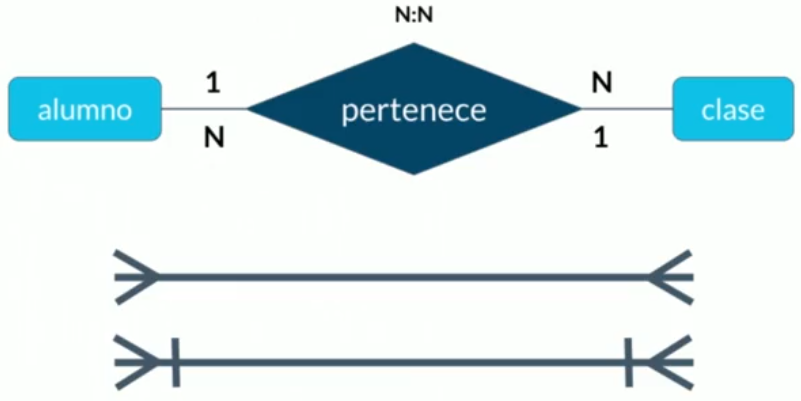
\includegraphics[scale=0.45]{./Pictures/018_card_N_N.png}
\end{figure}

\newpage

%% Clase 7
\section{Diagrama ER}%
Un diagrama es como un mapa y nos ayuda a entender cuáles son las entidades con
las que vamos a trabajar, cuáles son sus relaciones y qué papel van a jugar en
las aplicaciones de la base de datos.

\begin{figure}[h!]
    \centering
      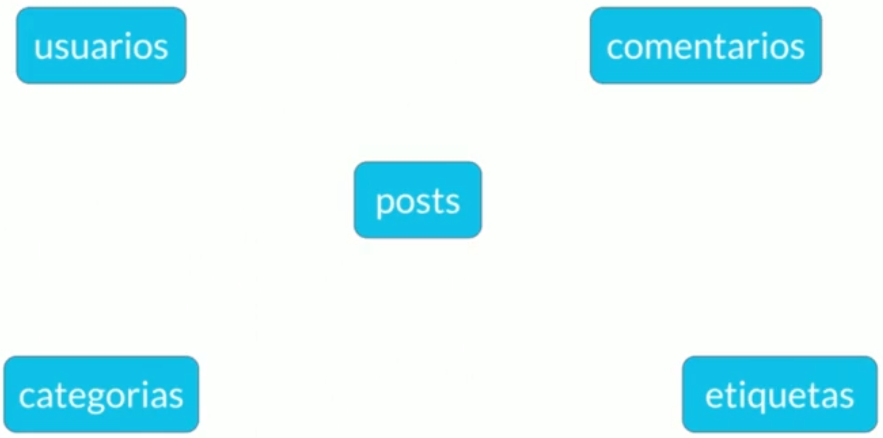
\includegraphics[scale=0.5]{./Pictures/018_DiagramaER.png}
\end{figure}

\begin{figure}[h!]
    \centering
      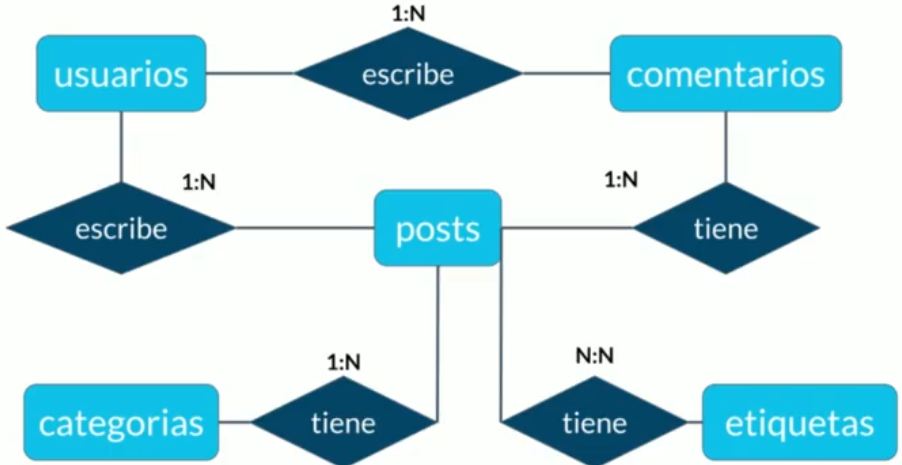
\includegraphics[scale=0.5]{./Pictures/019_diagrama_ER.png}
\end{figure}

%% Clase 8
\section{Diagrama Físico: tipos de datos y constraints}%
Para llevar a la práctica un diagrama debemos ir más alla y darle detalle con
parámetros como:

\textbf{Tipos de datos:}
\begin{itemize}
  \item \textbf{Texto:} CHAR(n), VARCHAR(n), TEXT.
  \item \textbf{Números:} INTEGER, BIGINT, SMALLINT, DECIMAL(n,s), NUMERIC(n,s)
  \item \textbf{Fecha/hora:} DATE, TIME, DATETIME, TIMESTAMP
  \item \textbf{Lógicos:} BOOLEAN
\end{itemize}

\begin{figure}[h!]
    \centering
      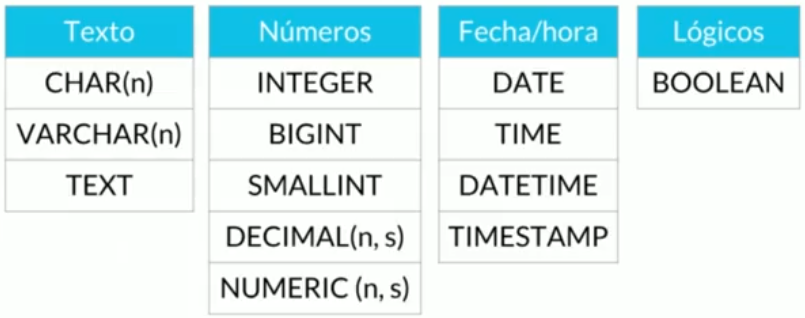
\includegraphics[scale=0.45]{./Pictures/020_tipos_datos.png}
\end{figure}

\newpage

\textbf{Constraints (Restricciones)}
\begin{itemize}
  \item \textbf{NOT NULL:} Se asegura que la columna no tenga valores nulos
  \item \textbf{UNIQUE:} Se asegura que cada valor en la columna no se repita
  \item \textbf{PRIMARY KEY:} Es una combinación de NOT NULL y UNIQUE
  \item \textbf{FOREIGN KEY:} Identifica de manera única una tupla en otra tabla
  \item \textbf{CHECK:} Se asegura que el valor en la columna cumpla una condición dada
  \item \textbf{DEFAULT:} Coloca un valor por defecto cuando no hay un valor especificado
  \item \textbf{INDEX:} Se crea por columna para permitir búsquedas más rápidas
\end{itemize}

\begin{figure}[h!]
    \centering
      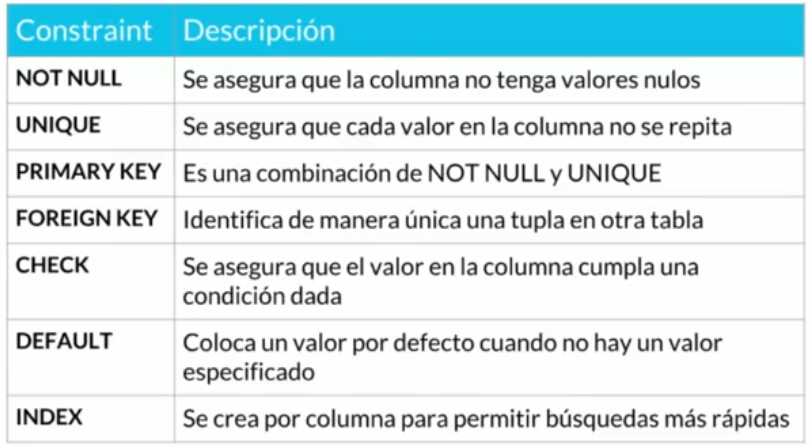
\includegraphics[scale=0.5]{./Pictures/021_constraints.png}
\end{figure}


%% Clase 9
\section{Diagrama Físico: normalización}%
La normalización como su nombre lo indica nos ayuda a dejar todo de una forma
normal. Esto obedece a las 12 reglas de \textbf{Codd} y nos permiten separar
componentes en la base de datos:\\

\begin{itemize}
  \item \textbf{Primera forma normal (1FN):} Atributos atómicos (Sin campos repetidos).
  \item \textbf{Segunda forma normal (2FN):} Cumple 1FN y cada campo de la
    tabla debe depender de una clave única.
  \item \textbf{Tercera forma normal (3FN):} Cumple 1FN y 2FN y los campos que
    NO son clave, NO deben tener dependencias.
  \item \textbf{Cuarta forma normal (4FN):} Cumple 1FN, 2FN, 3FN y los campos
    multivaluado se indentifican por una clave única
\end{itemize}

Por ejemplo la siguiente tabla muestra datos \textbf{sin normalizar}:

\begin{figure}[h!]
    \centering
      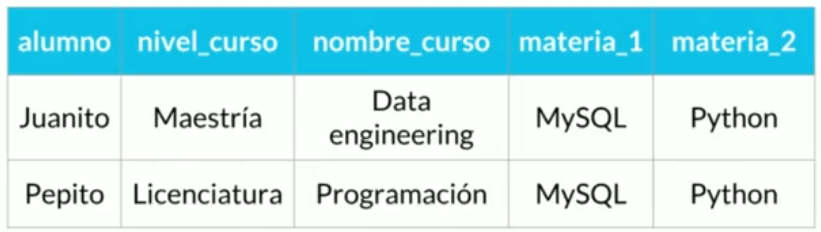
\includegraphics[scale=0.45]{./Pictures/022_sin_normalizar.png}
\end{figure}

Como se verifica en esta tabla, hay campos repetidos materia1 y materia2 que al
fin y al cabo son materia y si se aplica la primera normal entonces tendremos
lo siguiente:

\newpage

\begin{figure}[h!]
    \centering
      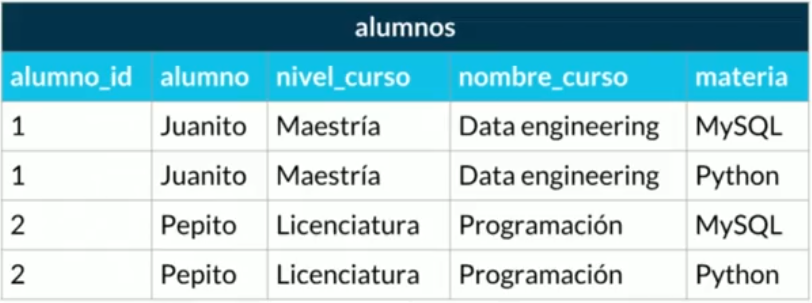
\includegraphics[scale=0.45]{./Pictures/023_primera_normal.png}
\end{figure}

Luego aplicando la segunda regla normal tendremos lo siguiente:
\begin{figure}[h!]
    \centering
      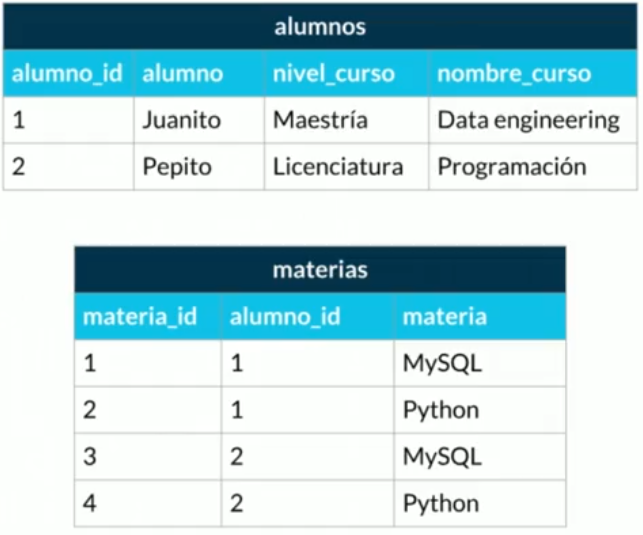
\includegraphics[scale=0.5]{./Pictures/024_segunda_normal.png}
\end{figure}

Ahora a estas tablas aplicaremos la tercera regla normal y obtendremos las siguientes:

\begin{figure}[h!]
    \centering
      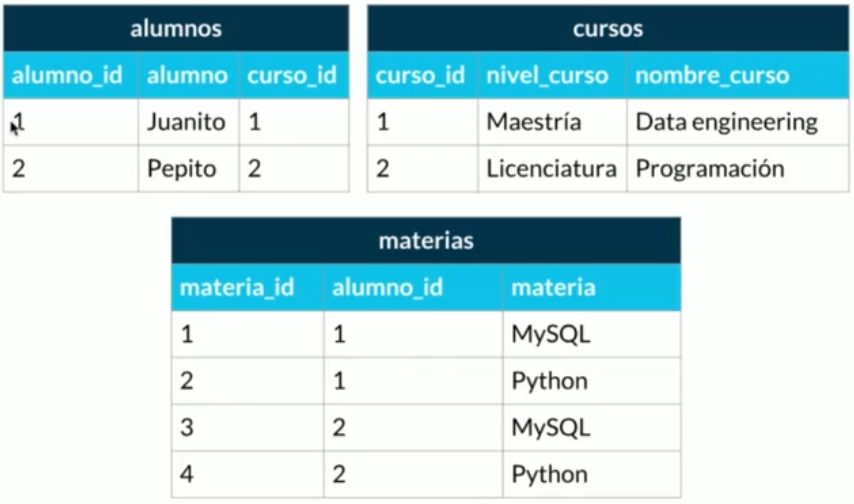
\includegraphics[scale=0.45]{./Pictures/025_tercera_normal.png}
\end{figure}

Finalmente con la cuarta forma normal obtendremos lo siguiente:

\begin{figure}[h!]
    \centering
      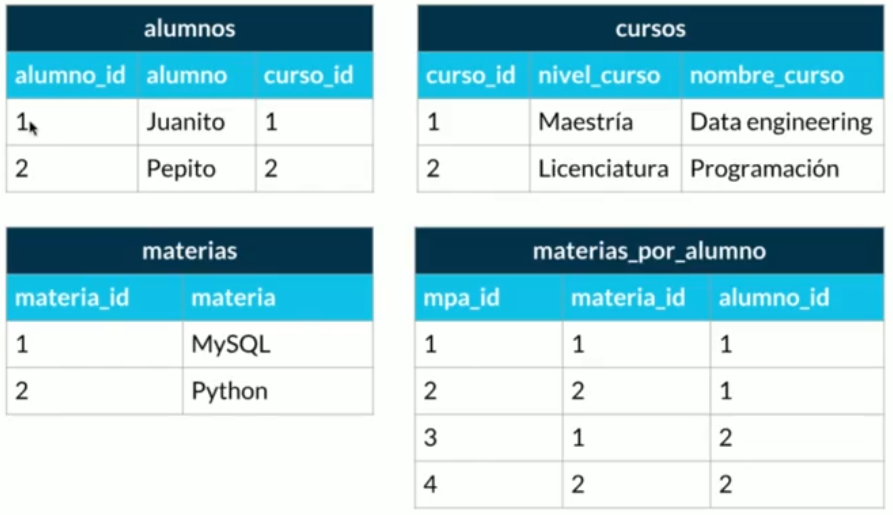
\includegraphics[scale=0.45]{./Pictures/026_cuarta_normal.png}
\end{figure}


%% Clase 10
\section{Diagrama Físico: normalizando Platziblog}%
Comencemos con el diagrama que ya teníamos de Platziblog. Aquí tenemos nuestras
entidades, relaciones y cardinalidad que existe entre ellos.\\

\begin{figure}[h!]
    \centering
      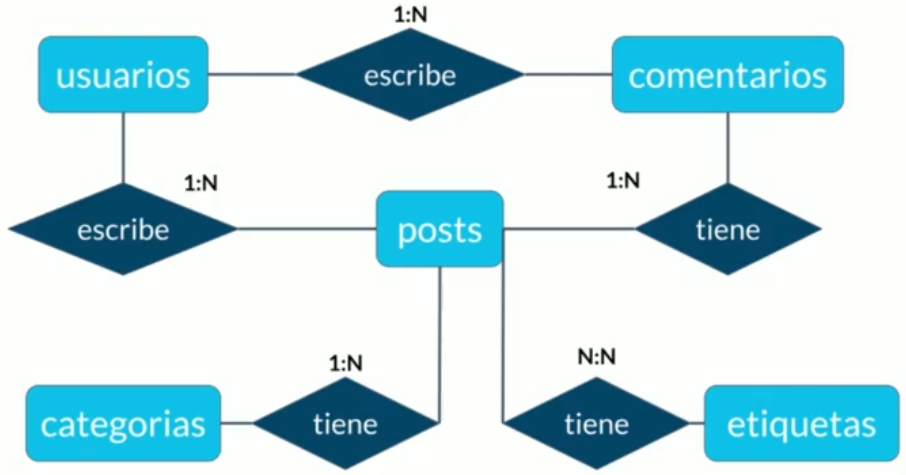
\includegraphics[scale=0.45]{./Pictures/027_diagramaER.png}
\end{figure}

Ahora veamos el diagrama físico:

\begin{figure}[h!]
    \centering
      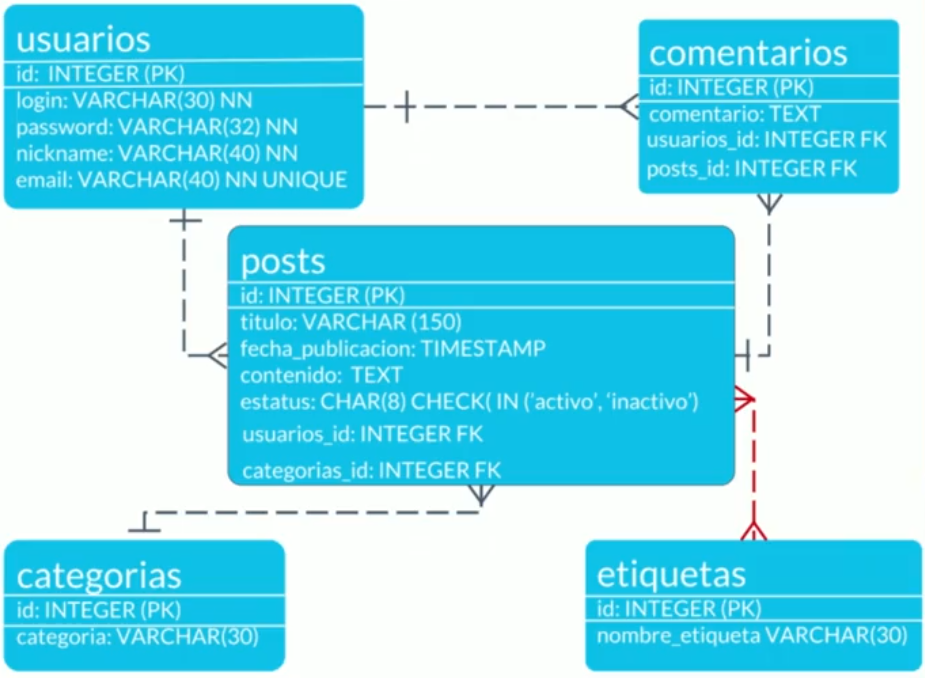
\includegraphics[scale=0.45]{./Pictures/028_diagrama_fisico.png}
\end{figure}

Como se ve en el diagrama en cada relación de 1 a muchos, al que tiene muchos
se le agrega el \textbf{Foreign Key} de la entidad que solo tiene uno en la
relación de cardinalidad. Sin embargo hay que tener en consideración la
relación de muchos a muchos que se verifica entre \textbf{posts} y
\textbf{etiquetas} ya que tiene un trato diferente al relacionarlos.


%% Clase 11
\section{Formas normales en DB relacionales}%
La normalización en las bases de datos relacionales es uno de esos temas, que
por un lado es sumamente importante y por el otro suena algo esotérico. Vamos a
tratar de entender las formas normales (FN) de una manera simple para que
puedas aplicarlas en tus proyectos profesionales.\\

\textbf{Primera Forma Normal (1FN)}\\
Esta FN nos ayuda a eliminar los valores repetidos y no atómicos dentro de una
base de datos.\\

Formalmente, una tabla está en primera forma normal si:

\begin{itemize}
  \item Todos los atributos son atómicos. Un atributo es atómico si los
    elementos del dominio son simples e indivisibles.
  \item No debe existir variación en el número de columnas.
  \item Los campos no clave deben identificarse por la clave (dependencia
    funcional)
  \item Debe existir una independencia del orden tanto de las filas como de las
    columnas; es decir, si los datos cambian de orden no deben cambiar sus
    significados.
\end{itemize}

Se traduce básicamente a que si tenemos campos compuestos como por ejemplo
"nombre\_completo" que en realidad contiene varios datos distintos, en este
caso podrían ser "nombre", "apellido\_paterno", "apellido\_materno", etc.\\

También debemos asegurarnos que las columnas son las mismas para todos los
registros, que no haya registros con columnas de más o de menos.\\

Todos los campos que no se consideran clave deben depender de manera única por
el o los campos que si son clave.\\

Los campos deben ser tales que si reordenamos los registros o reordenamos las
columnas, cada dato no pierda el significado.\\

\textbf{Segunda Forma Normal (2FN)}\\
Esta FN nos ayuda a diferenciar los datos en diversas entidades.\\

Formalmente, una tabla está en segunda forma normal si:
\begin{itemize}
  \item Está en 1FN
  \item Si los atributos no forman parte de ninguna clave dependen de forma
    completa de la clave principal. Es decir, que no existen dependencias
    parciales.
  \item Todos los atributos que no son clave principal deben depender
    únicamente de la clave principal.
\end{itemize}

Lo anterior quiere decir que si tenemos datos que pertenecen a diversas
entidades, cada entidad debe tener un campo clave separado. Por ejemplo.

\begin{figure}[h!]
    \centering
      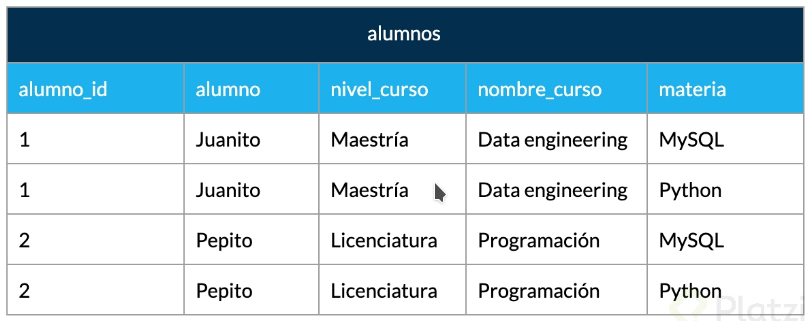
\includegraphics[scale=0.5]{./Pictures/029_normalizacion.png}
\end{figure}

En la tabla anterior tenemos por lo menos dos entidades que debemos separar
para que cada una dependa de manera única de su campo llave o ID. En este caso
las entidades son alumnos por un lado y materias por el otro, ya que una
materia. En el ejemplo anterior, quedaría de la siguiente manera:

\begin{figure}[h!]
    \centering
      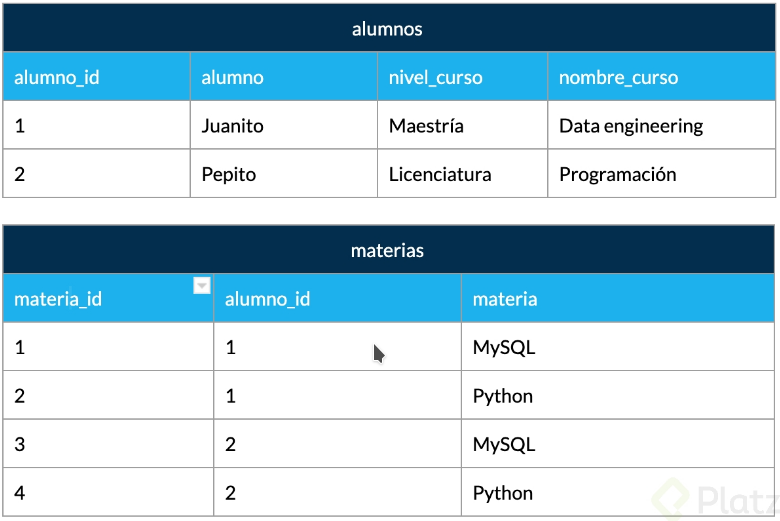
\includegraphics[scale=0.5]{./Pictures/030_normalizacion.png}
\end{figure}

\textbf{Tercera Forma Normal (3FN)}
Esta FN nos ayuda a separar conceptualmente las entidades que no son
dependientes.\\

Formalmente, una tabla está en tercera forma normal si:

Se encuentra en 2FN. No existe ninguna dependencia funcional transitiva en los
atributos que no son clave.

Esta FN se traduce en que aquellos datos que no pertenecen a la entidad deben
tener una independencia de las demás y debe tener un campo clave propio.
Continuando con el ejemplo anterior, al aplicar la 3FN separamos la tabla
alumnos ya que contiene datos de los cursos en ella quedando de la siguiente
manera.

\begin{figure}[h!]
    \centering
      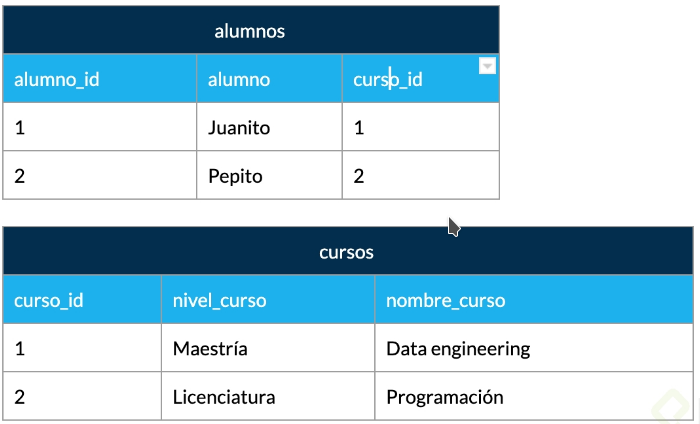
\includegraphics[scale=0.5]{./Pictures/031_normalizacion.png}
\end{figure}

\begin{figure}[h!]
    \centering
      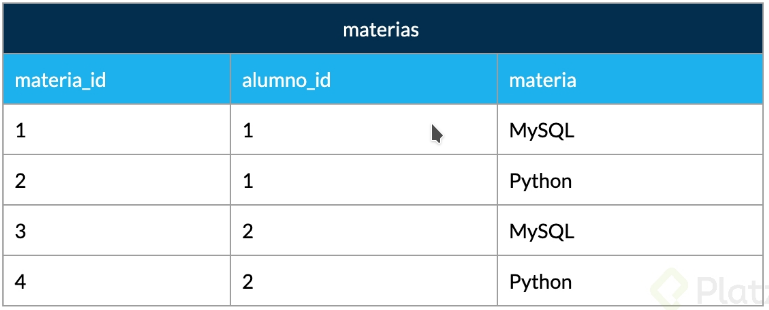
\includegraphics[scale=0.5]{./Pictures/032_normalizacion.png}
\end{figure}

\textbf{Cuarta Forma Normal (4FN)}\\
Esta FN nos trata de atomizar los datos multivaluados de manera que no tengamos
datos repetidos entre rows.\\

Formalmente, una tabla está en cuarta forma normal si:
\begin{itemize}
  \item Se encuentra en 3FN
  \item Los campos multivaluados se indentifican por una clave única
\end{itemize}

Esta FN trata de eliminar registros duplicados en una entidad, es decir que
cada registro tenga un contenido único y de necesitar repetir la data en los
resultados se realiza a través de claves foráneas.\\

Aplicando al ejemplo anterior la tabla materia se independiza y se relaciona
con el alumno a través de una tabla transitiva o pivote, de tal manera que si
cambiamos el nombre de la materia solamente hay que cambiarla una vez y se
propagará a cualquier referencia que haya de ella.

\begin{figure}[h!]
    \centering
      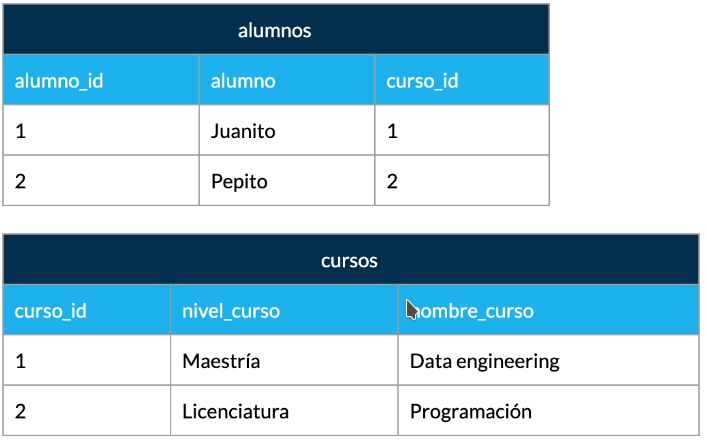
\includegraphics[scale=0.5]{./Pictures/033_normalizacion.png}
\end{figure}

\newpage

\begin{figure}[h!]
    \centering
      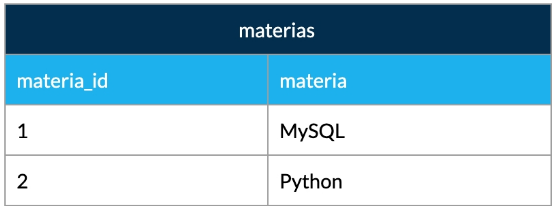
\includegraphics[scale=0.5]{./Pictures/034_normalizacion.png}
\end{figure}

\begin{figure}[h!]
    \centering
      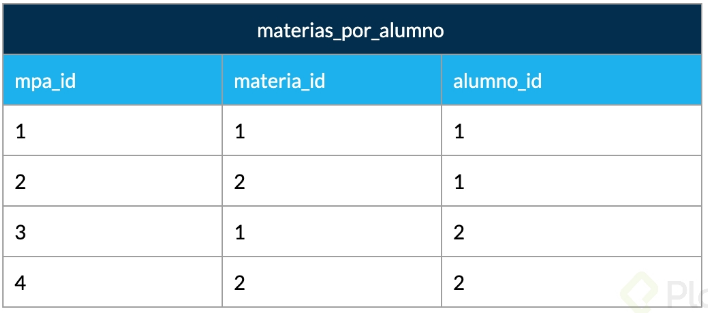
\includegraphics[scale=0.5]{./Pictures/035_normalizacion.png}
\end{figure}

De esta manera, aunque parezca que la infomación se multiplicó, en realidad la
descompusimos o normalizamos de manera que a un sistema le sea fácil de
reconocer y mantener la consistencia de los datos.\\

Algunos autores precisan una 5FN que hace referencia a que después de realizar
esta normalización a través de uniones (JOIN) permita regresar a la data
original de la cual partió.

\newpage

%% Clase 16
\section{Clientes Gráficos}%
\textbf{MySQL Workbench}: Abrimos nuestro cliente gráfico.
\begin{figure}[h!]
  \centering
  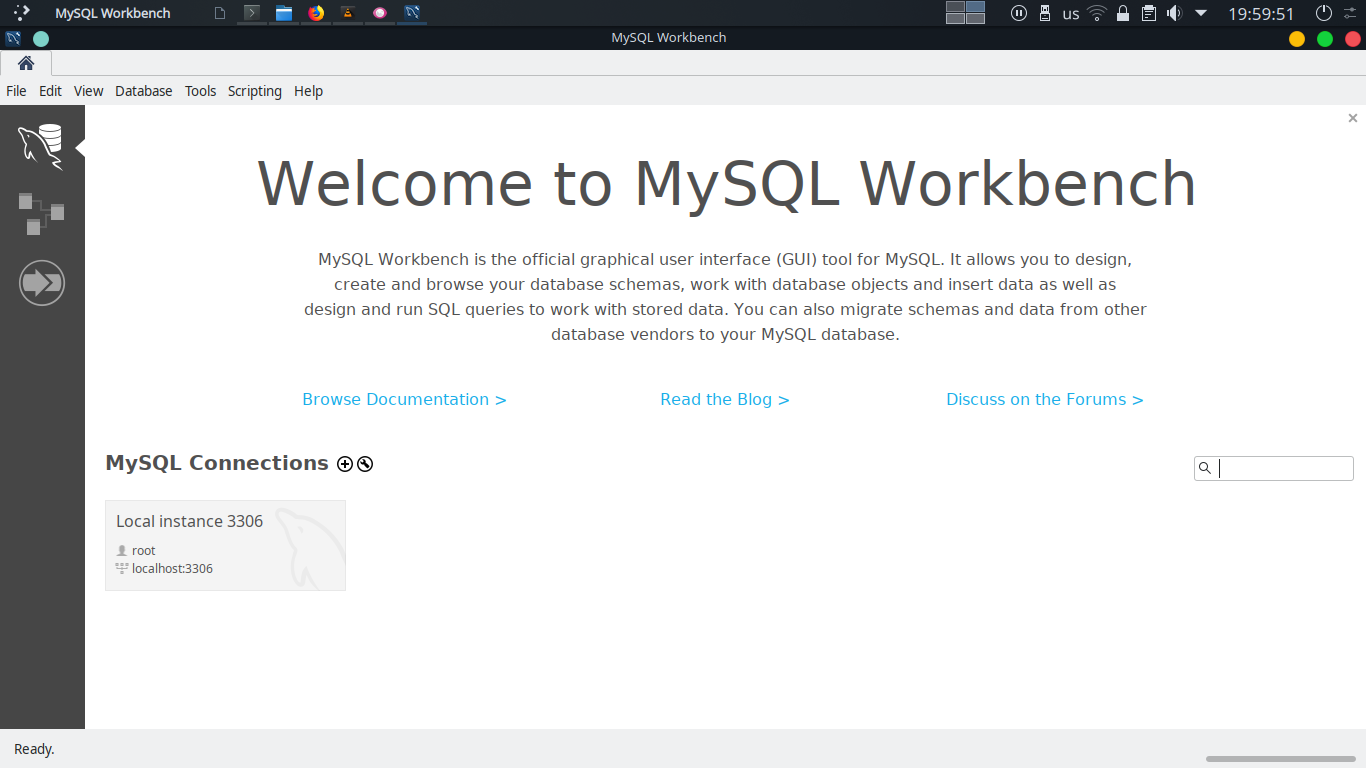
\includegraphics[scale=0.47]{./Pictures/036_workbench.png}
\end{figure}

En la parte inferior nos podemos logear a una conexión, para lo cual nos pedirá
la contraseña para root configurada al momeno de isntalar la base de datos.\\

\begin{figure}[h!]
  \centering
  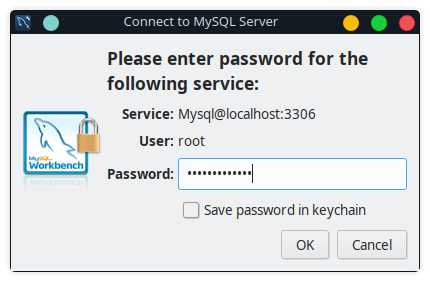
\includegraphics[scale=0.65]{./Pictures/037_local_instance_log.png}
\end{figure}

Veremos como se muestra nuestra área de trabajo y podemos crear un nuevo
esquema de la siguiente manera:

\begin{figure}[h!]
  \centering
  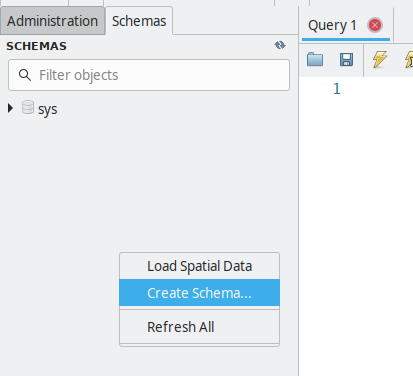
\includegraphics[scale=0.68]{./Pictures/038_create_schema.png}
\end{figure}

\begin{figure}[h!]
  \centering
  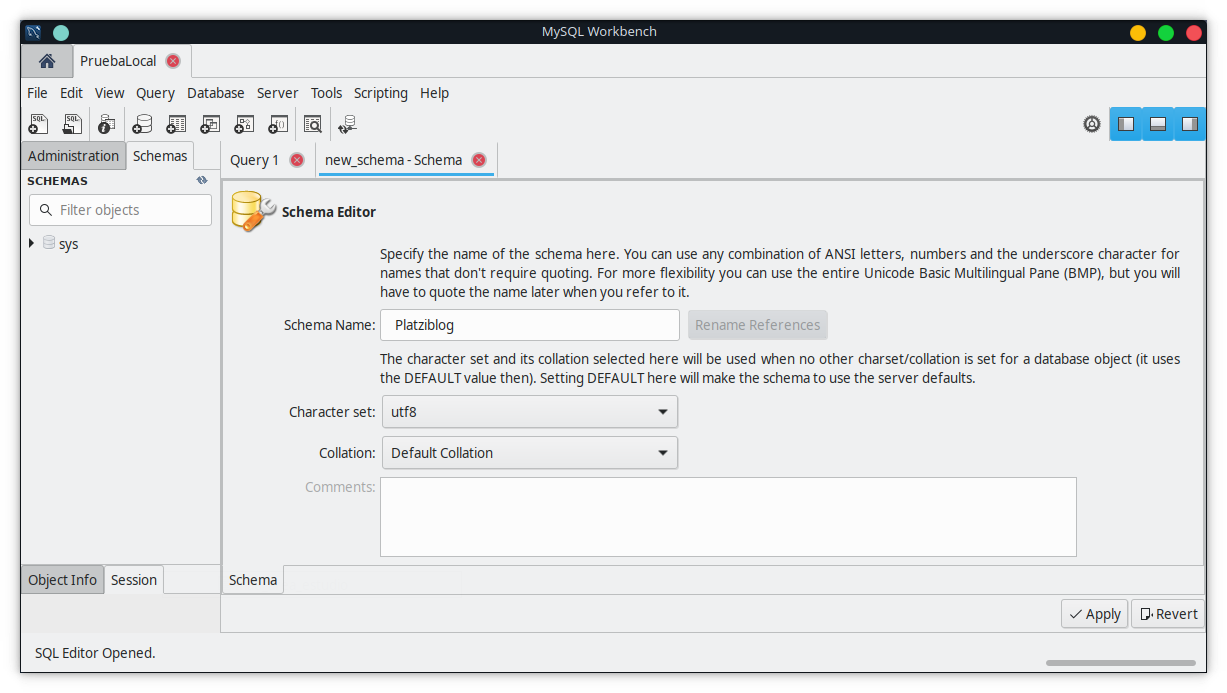
\includegraphics[scale=0.55]{./Pictures/039_create_schema.png}
\end{figure}

\newpage

\begin{figure}[h!]
  \centering
  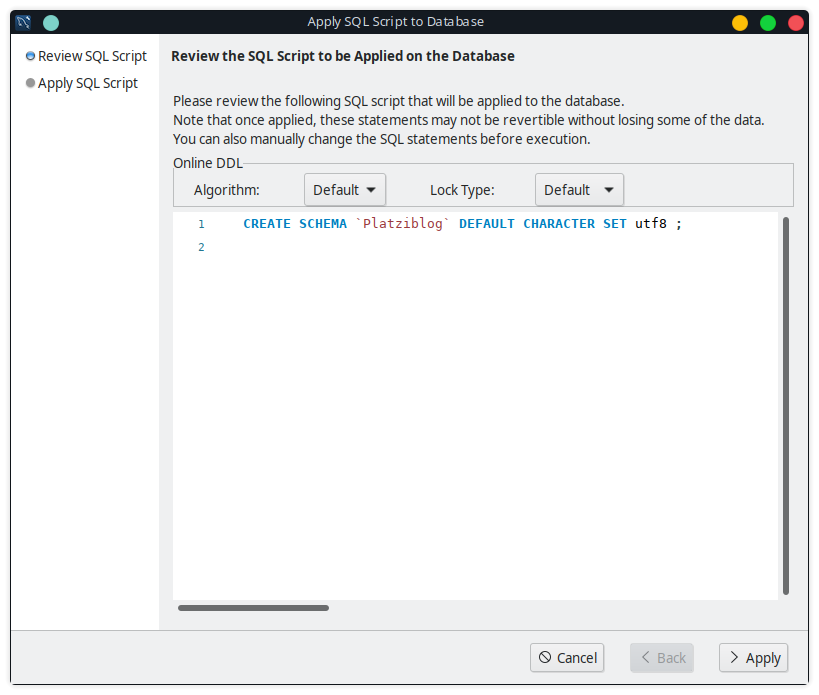
\includegraphics[scale=0.65]{./Pictures/040_create_schema.png}
\end{figure}

\newpage

Luego como vemos en la parte izquierda de nuestra ventana, observaremos el
esquema con el que podremos estar trabajando con diferentes opciones.

\begin{figure}[h!]
  \centering
  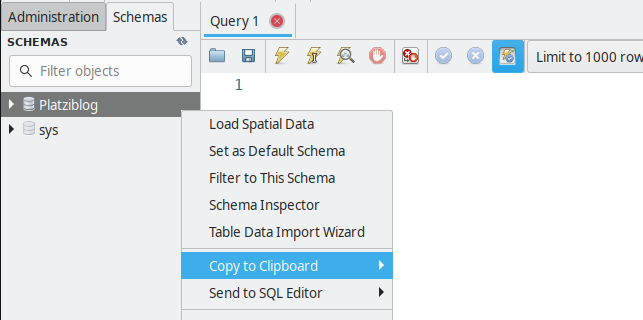
\includegraphics[scale=0.65]{./Pictures/041_create_schema.png}
\end{figure}



%% Clase 17
\section{Servicios administrados}%
Hoy en día muchas empresas ya no tienen instalados en sus servidores los
\textbf{RDBMS} sino que los contratan a otras personas. Estos servicios
administrados cloud te permiten concentrarte en la base de datos y no en su
administración y actualización.\\

Por ejemplo Google Cloud Platform, AWS o Azure te brindan estas posibilidades.

\newpage

%% Clase 18
\section{Historia de SQL}%
\textbf{SQL} significa Structured Query Language y tiene una estructura clara y
fija. Su objetivo es hacer un solo lenguaje para consultar cualquier manejador
de bases de datos volviendose en un gran estándar.\\

Ahora existe el \textbf{NOSQL} o Not Only Structured Query Language que
significa que no sólo se utiliza SQL. Las bases de datos no relacionales.


%% Clase 19
\section{DDL Create}%
\textbf{SQL} tiene dos grandes sublenguajes:\\
\textbf{DDL} o Data Definition Language que nos ayuda a crear la estructura de
una base de datos.\\
Existen 3 grandes comandos:
\begin{itemize}
  \item Create: Nos ayuda a crear bases de datos, tablas, vistas, índices, etc.
  \item Alter: Ayuda a alterar o modificar entidades.
  \item Drop: Nos ayuda a borrar. Hay que tener cuidado al utilizarlo.
\end{itemize}

\textbf{3 objetos que manipularemos con el lenguaje DDL:}
\begin{itemize}
  \item Database o bases de datos
  \item Table o tablas. Son la traducción a SQL de las entidades
  \item View o vistas: Se ofrece la proyección de los datos de la base de datos
    de forma entendible.
\end{itemize}

Vamos a crear un \textbf{schema} llamado Platziblog usando nuestro cliente gráfico.\\
\begin{figure}[h!]
  \centering
  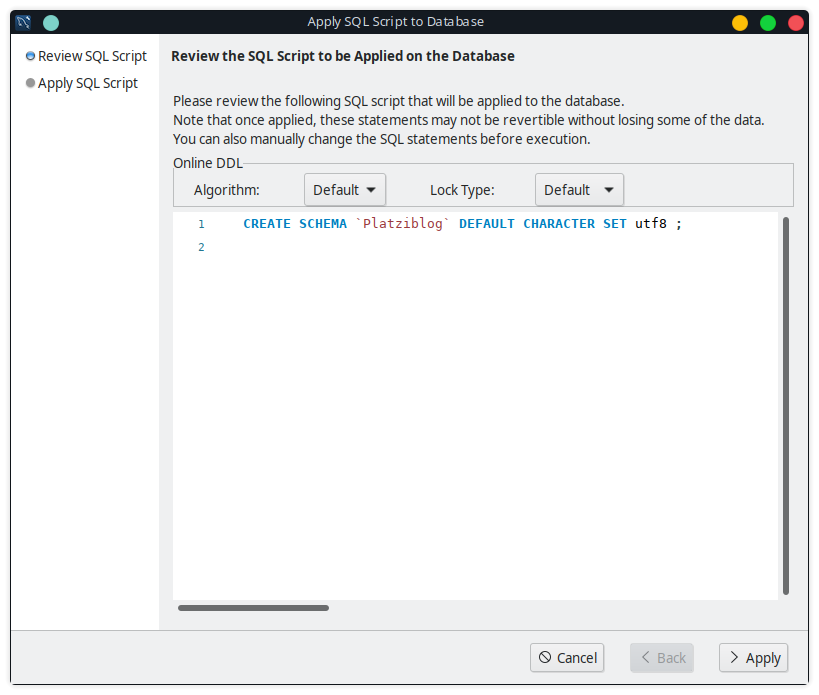
\includegraphics[scale=0.65]{./Pictures/040_create_schema.png}
\end{figure}

Como vemos \textbf{CREATE} es nuestro comando de creación.

\newpage

Ahora vamos a usar nuestro esquema usando nuestro cliente gráfico.\\

\begin{figure}[h!]
  \centering
  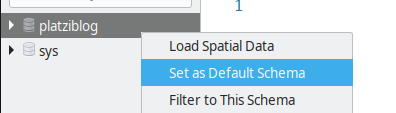
\includegraphics[scale=0.65]{./Pictures/043_use_database.png}
\end{figure}

Esto es equivalente a nuestro comando \textbf{USE DATABASE}\\

Por último vamos a crear una tabla:

\begin{figure}[h!]
  \centering
  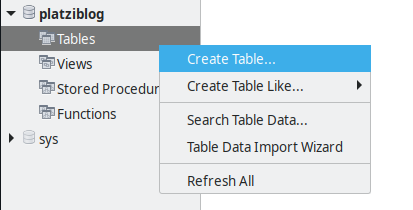
\includegraphics[scale=0.65]{./Pictures/044_create_table.png}
\end{figure}

Agregamos cada uno de nuestros campos.\\

\begin{figure}[h!]
  \centering
  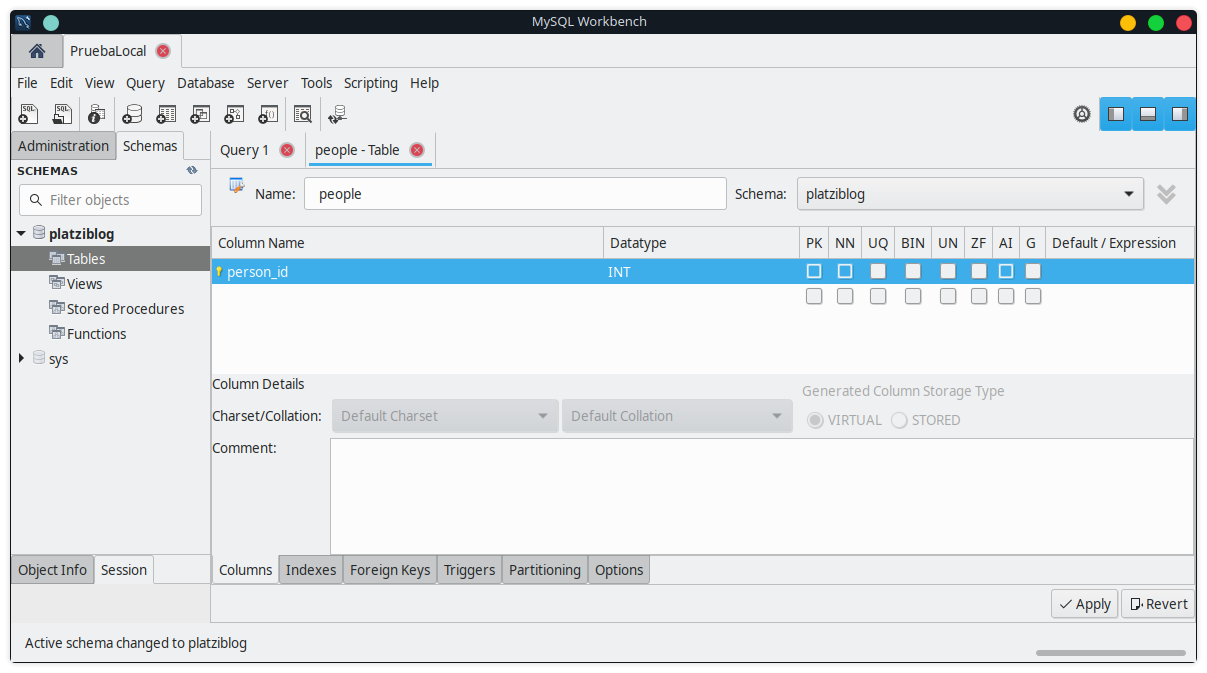
\includegraphics[scale=0.55]{./Pictures/045_person_id.png}
\end{figure}

\newpage
Por defecto nos da marcado el constraint PK (Primary Key) y NN (Not Null).
Podemos agregarle el constraint AI (Auto Increment) para que no tenga el mismo
id nunca.\\

\begin{figure}[h!]
  \centering
  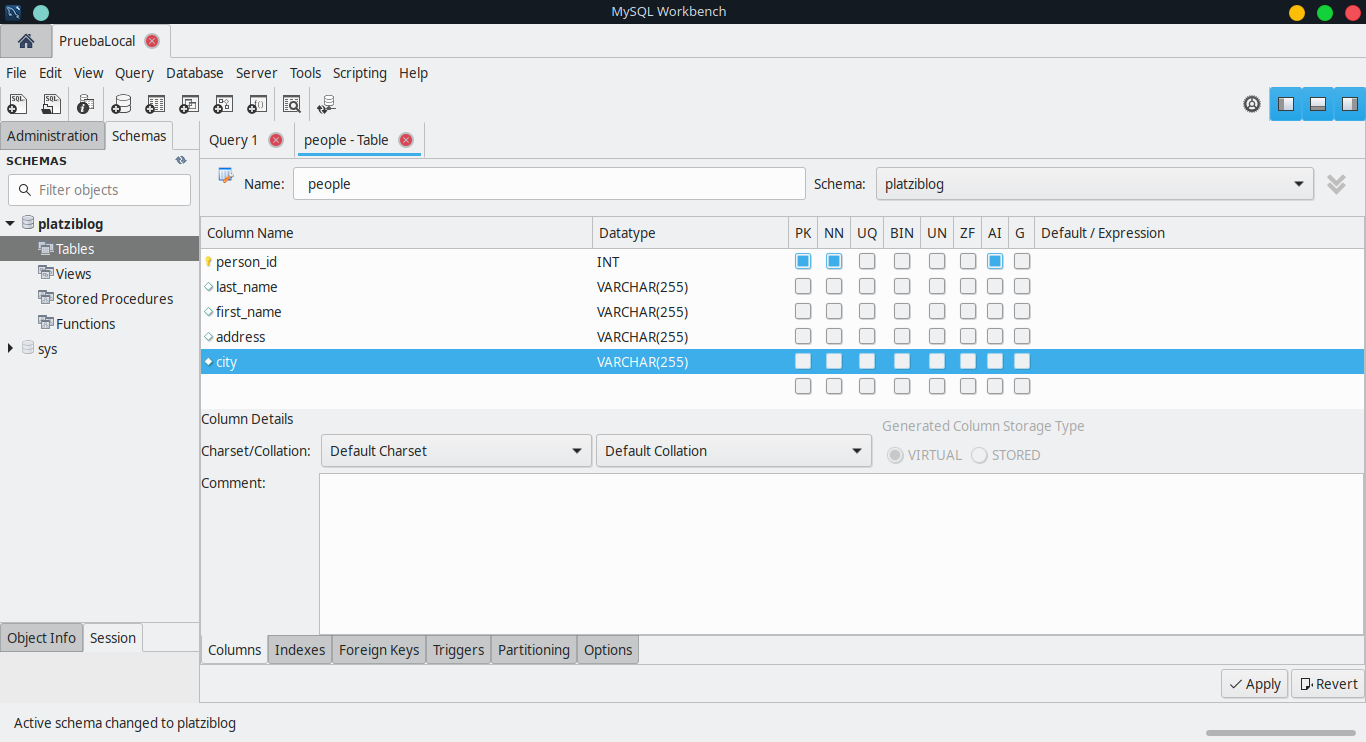
\includegraphics[scale=0.45]{./Pictures/046_people_atributos.png}
\end{figure}

\begin{figure}[h!]
  \centering
  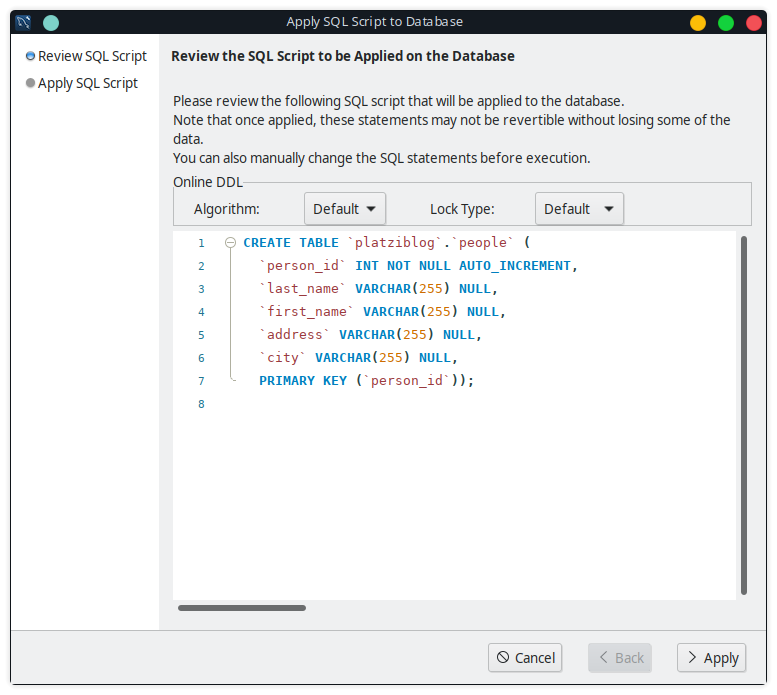
\includegraphics[scale=0.65]{./Pictures/047_people_apply.png}
\end{figure}

\newpage
Vamos hacer nuestra primera consulta para que veas nuestra tabla quedó bien hecha.\\

\begin{figure}[h!]
  \centering
  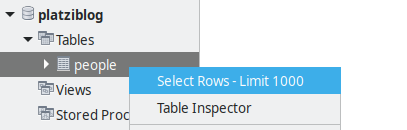
\includegraphics[scale=0.75]{./Pictures/048_selec.png}
\end{figure}

\begin{figure}[h!]
  \centering
  \includegraphics[scale=0.75]{./Pictures/049_select.png}
\end{figure}

Todo lo anterior se puede resumir en el siguiente código SQL:
\begin{minted}{mysql}
  CREATE DATABASE platziblog;
  USE platziblog;
  CREATE TABLE people (
    person_id INT NOT NULL AUTO_INCREMENT,
    first_name VARCHAR(255),
    last_name VARCHAR(255),
    address VARCHAR(255),
    city VARCHAR(255),
    PRIMARY KEY(person_id)
  );
  DESCRIBE people;
\end{minted}

Con \textbf{DESCRIBE people;} podemos ver una descripción de los campos
presentes en nuestra entidad people.\\

\textbf{Nota:} Para poder ver nuestras \textbf{databases} y nuestras
\textbf{tablas} en una terminal (sin cliente gráfico) se usan las siguientes
sentencias:

\begin{minted}{mysql}
  SHOW DATABASES;
  SHOW TABLES;
\end{minted}

Es necesario tener en cuenta que antes de usar \textbf{SHOW TABLES} deberá
estar en uso un esquema, esto se puede lograr con el comando \textbf{USE ...}

\begin{figure}[h!]
  \centering
  \includegraphics[scale=0.65]{./Pictures/143_ddl_create.png}
\end{figure}

\newpage
También ten en cuenta que en SQL las mayusculas y minúsculas no se discriminan,
pero su uso permite distinguir las instrucciones.

\newpage
%% Clase 20
\section{Vistas}%
Vamos a revisar la creación de vistas, tienen que ver con un concepto muy
avanzado y útil. Las vistas lo que hacen es tomar datos de la base de datos,
ponerlos en una forma presentable y convertirlas en algo que podamos consultar
de manera recurrente.\\

\begin{minted}{mysql}
  USE platziblog;
  CREATE VIEW platzi_people AS
  SELECT person_id, first_name FROM people;
\end{minted}

Ahora por ejemplo si seleccionamos con el siguiente comando:

\begin{minted}{mysql}
  SELECT * FROM platzi_people;
\end{minted}

Los Views toman datos de la base de datos, los hacen presentables y los
convierten en algo que podamos consultar de manera recurrente.

\begin{figure}[h!]
  \centering
  \includegraphics[scale=0.50]{./Pictures/146_ddl_create_vistas.png}
\end{figure}

%% Clase 21
\section{DDL alter}%
Este comando nos va a permitir modificar nuestra tabla. Por ejemplo agregar una
columna a nuestra tabla o el tipo de un campo, etc.

\begin{minted}{mysql}
  ALTER TABLE people
  ADD date_of_birth date;

  ALTER TABLE people
  CHANGE COLUMN date_of_birth date_of_birth year;

  ALTER TABLE people
  DROP COLUMN date_of_birth;
\end{minted}

\begin{figure}[h!]
  \centering
  \includegraphics[scale=0.5]{./Pictures/147_ddl_alter.png}
\end{figure}


%% Clase 21
\section{DDL drop}%
Esta puede ser la sentencia ¡más peligrosa!, sobre todo cuando somos
principiantes. Básicamente borra o desaparece de nuestra base de datos algún
elemento.

\begin{minted}{mysql}
  DROP VIEW platzi_people;
  DROP TABLE people;
  DROP DATABASE platziblog;
\end{minted}

\begin{figure}[h!]
  \centering
  \includegraphics[scale=0.75]{./Pictures/058_drop_table.png}
\end{figure}

\newpage

\begin{figure}[h!]
  \centering
  \includegraphics[scale=0.75]{./Pictures/059_drop_table_retriew.png}
\end{figure}

\begin{figure}[h!]
  \centering
  \includegraphics[scale=0.75]{./Pictures/060_drop_schema.png}
\end{figure}

\begin{figure}[h!]
  \centering
  \includegraphics[scale=0.75]{./Pictures/061_drop_database.png}
\end{figure}

\begin{figure}[h!]
  \centering
  \includegraphics[scale=0.65]{./Pictures/148_ddl_drop.png}
\end{figure}

%% Clase 22
\section{DML}%
\textbf{DML} trata del contenido de la base de datos. Son las siglas de Data
Manipulation Language y sus comandos son:
\begin{itemize}
  \item \textbf{Insert}: Inserta o agrega nuevos registros a la tabla.
  \item \textbf{Update}: Actualiza o modifica los datos que ya existen.
  \item \textbf{Delete}: Esta setencia es riesgosa porque puede borrar el contenido de una tabla.
  \item \textbf{Select}: Trae información de la base de datos.
\end{itemize}

\vspace{0.4cm}
\textbf{Insert}\\
Se puede realizar este procedimiento de manera muy sencilla usando un cliente gráfico como Workbench.\\
\begin{figure}[h!]
  \centering
  \includegraphics[scale=0.75]{./Pictures/149_dml_insert_workbench.png}
\end{figure}

No olvides dar clic en \textbf{Apply} para que se guarden los cambios y seguir
los pasos en los que Workbench te guía. La ventaja de usar un cliente gráfico
radica en que éste te muestra las instrucciones SQL que usa en cada
procedimiento antes de aplicar cambios.\\

Veamos un ejemplo de la instrucción SQL usada para insertar:
\begin{minted}{mysql}
  INSERT INTO people (last_name, first_name, address, city)
  VALUES ('Hernández', 'Laura', 'Calle 21', 'Monterrey');
\end{minted}

\newpage

\begin{figure}[h!]
  \centering
  \includegraphics[scale=0.75]{./Pictures/150_dml_insert_console.png}
\end{figure}

Recuerda que en Workbench es posible ejecutar comandos SQL usando su Editor de
Scripts.

\begin{figure}[h!]
  \centering
  \includegraphics[scale=0.75]{./Pictures/062_insert.png}
\end{figure}

\vspace{0.4cm}

\textbf{Update}\\
Tiene que ver con actualizar o modificar los datos que ya tenemos.
\begin{minted}{mysql}
  UPDATE people
  SET last_name = 'Chávez', city = 'Mérida'
  WHERE person_id = 1;

  UPDATE people
  SET first_name = 'Juan'
  WHERE city = 'Mérida';

  UPDATE people
  SET first_name = 'Juan';
\end{minted}

\newpage

\begin{figure}[h!]
  \centering
  \includegraphics[scale=0.5]{./Pictures/151_dml_update_terminal.png}
\end{figure}

Se debe tener cuidado al usar update: es recomendable filtrar usando el
\textbf{primary key} que identifica a un registro en específico para no hacer
cambios masivos y perder información. Por otro lado el uso de un cliente
gráfico brinda una ventaja ya que genera advertencias antes de realizar algún
cambio para no perder información por realizar mal estas instrucciones.\\

\vspace{0.4cm}

\textbf{Delete}\\
Igual que DROP que vimos en el lenguaje DDL, ésta es una sentencia DML que
también es bastante riesgosa porque puede borrar el contenido de una tabla.

\begin{minted}{mysql}
  DELETE FROM people
  WHERE person_id = 1;

  DELETE FROM people;
\end{minted}

\vspace{0.4cm}

\textbf{Select}\\
Nos trae información de la base de datos, nos puede servir para generar una
vista.
\begin{minted}{mysql}
  SELECT first_name, last_name
  FROM people;
\end{minted}

\begin{figure}[h!]
  \centering
  \includegraphics[scale=0.65]{./Pictures/064_select.png}
\end{figure}

\newpage

\begin{figure}[h!]
  \centering
  \includegraphics[scale=0.65]{./Pictures/152_dml_select_delete.png}
\end{figure}


%% Clase 23
\section{¿Qué tan estandard es SQL?}%
La utilidad más grande de \textbf{SQL} fue unificar la forma en la que pensamos
y hacemos preguntas a un repositorio de datos. Ahora que nacen nuevas bases de
datos igualmente siguen tomando elementos de \textbf{SQL}.\\

Por ejemplo veamos los comandos usados en \textbf{mysql}.
\begin{figure}[h!]
  \centering
  \includegraphics[scale=0.75]{./Pictures/065_mysql.png}
\end{figure}

\newpage

También se pueden usar los mismos comando SQL en \textbf{postgresql}.
\begin{figure}[h!]
  \centering
  \includegraphics[scale=0.50]{./Pictures/066_postgresql.png}
\end{figure}

%% Clase 24
\section{Creando Platziblog: tablas independientes}%
\begin{itemize}
  \item Una buena práctica es comenzar creando las entidades que no tienen una
    llave foránea.
  \item Generalmente en los nombres de bases de datos se evita usar eñes o
    acentos para evitar problemas en los manejadores de las bases de datos.
\end{itemize}

\begin{minted}{mysql}
  /* Creacion de la base de datos platziblog */
  CREATE DATABASE platziblog DEFAULT CHARACTER SET uft8;
  /* Linea para utilizar platziblog */
  USE platziblog;
  
  /* Construccion de tablas independientes */
  CREATE TABLE categorias (
    id INT NOT NULL AUTO_INCREMENT,
    nombre_categoria VARCHAR(30),
    PRIMARY KEY (id)
  );

  CREATE TABLE etiquetas (
    id INT NOT NULL AUTO_INCREMENT,
    nombre_etiqueta VARCHAR(30),
    PRIMARY KEY (id)
  );

  CREATE TABLE usuarios (
    id INT NOT NULL AUTO_INCREMENT,
    login VARCHAR(30) NOT NULL,
    password VARCHAR(32) NOT NULL,
    nickname VARCHAR(40) NOT NULL,
    email VARCHAR(40) NOT NULL UNIQUE,
    PRIMARY KEY(id)
  );
\end{minted}

Esto lo podemos hacer a través de nuestro cliente gráfico o por consola como se puede observar.

\begin{figure}[h!]
  \centering
  \includegraphics[scale=0.50]{./Pictures/067_platziblog_ti.png}
\end{figure}

%% Clase 25
\section{Creando Platziblog: tablas dependientes}%
El comando "cascade" sirve para que cada que se haga un update en la tabla
principal, se refleje también en la tabla en la que estamos creando la
relación.\\

Vamos a crear la tabla \textbf{posts}:\\

\begin{minted}{mysql}
  CREATE TABLE posts (
    id INT NOT NULL AUTO_INCREMENT,
    titulo VARCHAR(130),
    fecha_publicacion TIMESTAMP,
    contenido TEXT,
    estatus CHAR(8) DEFAULT 'activo',
    usuario_id INT,
    categoria_id INT,
    PRIMARY KEY (id)
  );
\end{minted}

\newpage

Luego configuramos sus Foreign Keys, que en este caso son dos:\\

\begin{minted}{mysql}
  ALTER TABLE posts
  ADD INDEX fk_posts_usuarios_idx (usuario_id);

  ALTER TABLE posts
  ADD CONSTRAINT fk_posts_usuarios
    FOREIGN KEY (usuario_id)
    REFERENCES platziblog.usuarios(id)
    ON UPDATE cascade;

  ALTER TABLE posts
  ADD INDEX fk_posts_categorias_idx (categoria_id);

  ALTER TABLE posts
  ADD CONSTRAINT fk_posts_categorias
    FOREIGN KEY (categoria_id)
    REFERENCES categorias (id);
\end{minted}

Usando el Workbench sería así:\\

\begin{figure}[h!]
  \centering
  \includegraphics[scale=0.55]{./Pictures/068_fk.png}
\end{figure}

\begin{figure}[h!]
  \centering
  \includegraphics[scale=0.55]{./Pictures/070_fk.png}
\end{figure}

No olvides dar clic en \textbf{Apply} para guardar los cambios. Ahora veamos
como se realiza por terminal (sin cliente gráfico):\\

\begin{figure}[h!]
  \centering
  \includegraphics[scale=0.60]{./Pictures/153_platziblog_t_dependientes.png}
\end{figure}

\newpage

Creamos ahora la tabla \textbf{comentarios}:

\begin{minted}{mysql}
  CREATE TABLE comentarios (
    id INT NOT NULL AUTO_INCREMENT,
    cuerpo_comentario TEXT NOT NULL,
    usuario_id INT NOT NULL,
    post_id INT NOT NULL,
    PRIMARY KEY (id)
  );
\end{minted}

Añadimos sus \textbf{foreing keys}:

\begin{minted}{mysql}
  ALTER TABLE comentarios
    ADD INDEX fk_comentarios_usuarios_idx (usuario_id),
    ADD INDEX fk_comentarios_posts_idx (post_id);

  ALTER TABLE comentarios
    ADD CONSTRAINT fk_comentarios_usuarios
    FOREIGN KEY (usuario_id)
    REFERENCES platziblog.usuarios (id),
    ADD CONSTRAINT fk_comentarios_posts
    FOREIGN KEY (post_id)
    REFERENCES platziblog.posts (id);
\end{minted}

\newpage
Usando Workbench sería así:\\

\begin{figure}[h!]
  \centering
  \includegraphics[scale=0.55]{./Pictures/072_fk_comentarios.png}
\end{figure}

No olvides dar clic en \textbf{Apply} para guardar los cambios. Ahora veamos
como se realiza por terminal (sin cliente gráfico):\\

\begin{figure}[h!]
  \centering
  \includegraphics[scale=0.5]{./Pictures/154_platziblog_t_dependientes.png}
\end{figure}


%% Clase 26
\section{Creando Platziblog: tablas transitivas}%
Las tablas transitivas sirven como puente para unir dos tablas. No tienen
contenido semántico.\\

Creamos la tabla \textbf{posts\_etiqueta}:

\begin{minted}{mysql}
  CREATE TABLE posts_etiqueta (
    id INT NOT NULL AUTO_INCREMENT,
    post_id INT NOT NULL,
    etiqueta_id INT NOT NULL,
    PRIMARY KEY (id)
  );
\end{minted}

\newpage

Luego configuramos su Foreign Keys:

\begin{minted}{mysql}
  ALTER TABLE posts_etiqueta
    ADD INDEX fk_posts_etiqueta_posts_idx (post_id),
    ADD INDEX fk_posts_etiqueta_etiquetas_idx (etiqueta_id);

  ALTER TABLE posts_etiqueta
    ADD CONSTRAINT fk_posts_etiqueta_posts
    FOREIGN KEY (post_id)
    REFERENCES platziblog.posts (id),
    ADD CONSTRAINT fk_posts_etiqueta_etiquetas
    FOREIGN KEY (etiqueta_id)
    REFERENCES platziblog.etiquetas (id);
\end{minted}

Usando Workbench sería así:\\

\begin{figure}[h!]
  \centering
  \includegraphics[scale=0.55]{./Pictures/074_fk_pe_posts.png}
\end{figure}

No olvides dar clic en \textbf{Apply} para guardar los cambios. Ahora veamos
como se realiza por terminal (sin cliente gráfico):\\

\begin{figure}[h!]
  \centering
  \includegraphics[scale=0.5]{./Pictures/155_platziblog_t_transitiva.png}
\end{figure}

\newpage
Workbench tiene una herramienta llamada \textbf{Reverse Engineer} que nos
reproduce el esquema del cual nos basamos para crear nuestras tablas. Es útil
cuando llegas a un nuevo trabajo y quieres entender cuál fue la mentalidad que
tuvieron al momento de crear las bases de datos.

\begin{figure}[h!]
  \centering
  \includegraphics[scale=0.55]{./Pictures/076_reverse_engineer.png}
\end{figure}

\begin{figure}[h!]
  \centering
  \includegraphics[scale=0.55]{./Pictures/077_reverse_engineer.png}
\end{figure}

\begin{figure}[h!]
  \centering
  \includegraphics[scale=0.55]{./Pictures/077_select_schema.png}
\end{figure}

\newpage

\begin{figure}[h!]
  \centering
  \includegraphics[scale=0.55]{./Pictures/077_diag_fisico_workbench.png}
\end{figure}


%% Clase 27
\section{¿Por qué las consultas son tan importantes?}%
Las consultas o queries a una base de datos son una parte fundamental ya que
esto podría salvar un negocio o empresa.\\

Alrededor de las consultas a las bases de datos se han creado varias
especialidades como \textbf{ETL} o transformación de datos, \textbf{business
intelligence} e incluso \textbf{machine learning}.

%% Clase 28
\section{Estructura básica de un Query}%
Para poder realizar consultas a nuestra base de datos, primera vamos a
ingresarle datos de prueba. Para esto copiaremos el contenido del archivo que se encuentra en el siguiente :\\

Los queries son la forma en la que estructuramos las preguntas que se harán a
la base de datos. Transforma preguntas en sintaxis.\\

El query tiene básicamente 2 partes: \textbf{SELECT} y \textbf{FROM} y puede
aparecer una tercera como \textbf{WHERE}.\\

\textbf{Estructura básica de un Query}
\begin{figure}[h!]
  \centering
  \includegraphics[scale=0.55]{./Pictures/078_query.png}
\end{figure}

El asterisco (*) quiere decir que vamos a seleccionar todo sin filtrar campos, por ejemplo.

\begin{minted}{mysql}
  SELECT *
  FROM posts;
\end{minted}
\begin{figure}[h!]
  \centering
  \includegraphics[scale=0.55]{./Pictures/079_select_year.png}
\end{figure}

\begin{minted}{mysql}
  SELECT *
  FROM posts
  WHERE year(fecha_publicacion) > '2024';
\end{minted}

\begin{figure}[h!]
  \centering
  \includegraphics[scale=0.55]{./Pictures/079_select_ast.png}
\end{figure}



%% Clase 29
\section{SELECT}%
El select más básico es el siguiente:
\begin{minted}{mysql}
  SELECT *
  FROM posts;
\end{minted}

Ahora vamos a elegir solo algunos campos:
\begin{minted}{mysql}
  SELECT titulo, fecha_publicacion, estatus
  FROM posts;
\end{minted}
\begin{figure}[h!]
  \centering
  \includegraphics[scale=0.55]{./Pictures/080_select.png}
\end{figure}

Tambien podemos usar \textbf{AS} para modificar el nombre con el que se mostrarán los campos:
\begin{minted}{mysql}
  SELECT titulo AS encabezado, fecha_publicado AS publicado_en, estatus AS estado
  FROM posts;
\end{minted}
\begin{figure}[h!]
  \centering
  \includegraphics[scale=0.55]{./Pictures/081_select_as.png}
\end{figure}

\newpage

Podemos contar los registros usando \textbf{count()}:
\begin{minted}{mysql}
  SELECT count(*)
  FROM posts;
\end{minted}
\begin{figure}[h!]
  \centering
  \includegraphics[scale=0.75]{./Pictures/082_select_count.png}
\end{figure}


Y se puede modificar el nombre que se muestra por algo mas entendible usando
\textbf{AS}:
\begin{minted}{mysql}
  SELECT count(*) AS numero_posts
  FROM posts;
\end{minted}
\begin{figure}[h!]
  \centering
  \includegraphics[scale=0.75]{./Pictures/083_select_count_as.png}
\end{figure}


%% Clase 30
\section{FROM}%
\textbf{FROM} indica de dónde traer los datos y puede ayudar a hacer sentencias
y filtros complejos cuando se quieren unir tablas. La sentencia compañera que
nos ayuda con este proceso es \textbf{JOIN}.\\

Los diagramas de Venn son círculos que se tocan en algún punto para ver dónde
está la intersección de conjuntos. Ayudan mucho para poder formular la
sentencia \textbf{JOIN} de la manera adecuada dependiendo del query que se
quiere hacer.\\

\textbf{JOIN - Diferencia}\\
\begin{figure}[h!]
  \centering
  \includegraphics[scale=0.75]{./Pictures/084_join_diferencia.png}
\end{figure}

\newpage

\textbf{JOIN - Intersección}\\
\begin{figure}[h!]
  \centering
  \includegraphics[scale=0.75]{./Pictures/085_join_interseccion.png}
\end{figure}

\textbf{JOIN - Union - Diferencia simétrica}\\
\begin{figure}[h!]
  \centering
  \includegraphics[scale=0.75]{./Pictures/086_join_outer.png}
\end{figure}


%% Clase 31
\section{Utilizando la sentencia FROM}%
Vamos a empezar con \textbf{JOIN - Diferencia}:

\begin{figure}[h!]
  \centering
  \includegraphics[scale=0.75]{./Pictures/089_join_left.png}
\end{figure}

\begin{minted}{mysql}
  SELECT *
  FROM usuarios
  LEFT JOIN posts ON usuarios.id = posts.usuario_id;
\end{minted}

\begin{figure}[h!]
  \centering
  \includegraphics[scale=0.55]{./Pictures/087_join_left.png}
\end{figure}

\begin{figure}[h!]
  \centering
  \includegraphics[scale=0.55]{./Pictures/088_join_left_perezoso.png}
\end{figure}

\begin{figure}[h!]
  \centering
  \includegraphics[scale=0.75]{./Pictures/090_join_left_not_null.png}
\end{figure}

\begin{minted}{mysql}
  SELECT *
  FROM usuarios
  LEFT JOIN posts ON usuarios.id = posts.usuario_id
  WHERE posts.usuario_id IS NOT NULL;
\end{minted}

\begin{figure}[h!]
  \centering
  \includegraphics[scale=0.75]{./Pictures/093_join_left_not_null.png}
\end{figure}


\begin{figure}[h!]
  \centering
  \includegraphics[scale=0.75]{./Pictures/091_join_right.png}
\end{figure}

\begin{minted}{mysql}
  SELECT *
  FROM usuarios
  RIGHT JOIN posts ON usuarios.id = posts.usuario_id;
\end{minted}

\begin{figure}[h!]
  \centering
  \includegraphics[scale=0.75]{./Pictures/094_join_right.png}
\end{figure}


\begin{minted}{mysql}
  SELECT *
  FROM usuarios
  RIGHT JOIN posts ON usuarios.id = posts.usuario_id
  WHERE posts.usuario_id IS NOT NULL;
\end{minted}

\begin{figure}[h!]
  \centering
  \includegraphics[scale=0.75]{./Pictures/095_join_right_not_null.png}
\end{figure}

Ahora veremos la \textbf{Intersección}\\
\begin{figure}[h!]
  \centering
  \includegraphics[scale=0.75]{./Pictures/096_Interseccion.png}
\end{figure}

\begin{figure}[h!]
  \centering
  \includegraphics[scale=0.75]{./Pictures/099_inner.png}
\end{figure}


Ahora veremos la \textbf{Unión}

\begin{figure}[h!]
  \centering
  \includegraphics[scale=0.75]{./Pictures/097_union.png}
\end{figure}


%% Clase 32
\section{WHERE}%
\textbf{WHERE} es la sentencia que nos ayuda a filtar tuplas o registros
dependiendo de las características que elegimos.

Veamos por ejemplo una instrucción SELECT de posts:
\begin{figure}[h!]
  \centering
  \includegraphics[scale=0.75]{./Pictures/102_where.png}
\end{figure}

Y ahora agreguemos una sentencia WHERE con id con el que podemos hacer comparaciones de orden:
\begin{figure}[h!]
  \centering
  \includegraphics[scale=0.75]{./Pictures/103_where.png}
\end{figure}

\begin{figure}[h!]
  \centering
  \includegraphics[scale=0.75]{./Pictures/104_where.png}
\end{figure}

\begin{figure}[h!]
  \centering
  \includegraphics[scale=0.75]{./Pictures/107_where_id_dif.png}
\end{figure}


Podemos usar esta sentencia con el campo \textbf{estatus}, por ejemplo:
\begin{figure}[h!]
  \centering
  \includegraphics[scale=0.75]{./Pictures/105_where.png}
\end{figure}

\begin{figure}[h!]
  \centering
  \includegraphics[scale=0.75]{./Pictures/106_where_estatus.png}
\end{figure}

La propiedad \textbf{LIKE} nos ayuda a traer registros de los cuales conocemos
sólo una parte de la información.
\begin{figure}[h!]
  \centering
  \includegraphics[scale=0.75]{./Pictures/108_where_like.png}
\end{figure}

\begin{figure}[h!]
  \centering
  \includegraphics[scale=0.75]{./Pictures/109_where_like.png}
\end{figure}

\begin{figure}[h!]
  \centering
  \includegraphics[scale=0.75]{./Pictures/110_where_like.png}
\end{figure}

Nota: También podemos hacer comparaciones de orden con datos de tipo TIMESTAMP, por ejemplo:
\begin{figure}[h!]
  \centering
  \includegraphics[scale=0.75]{./Pictures/111_where_fecha.png}
\end{figure}

\begin{figure}[h!]
  \centering
  \includegraphics[scale=0.75]{./Pictures/112_where_fecha.png}
\end{figure}

La propiedad \textbf{BETWEEN} nos sirve para arrojar registros que estén en el
medio de dos. Por ejemplo los registros con id entre 20 y 30.

\begin{figure}[h!]
  \centering
  \includegraphics[scale=0.75]{./Pictures/114_where_id_between.png}
\end{figure}

También podemos usar between con fecha, por ejemplo:
\begin{figure}[h!]
  \centering
  \includegraphics[scale=0.75]{./Pictures/113_where_fecha_between.png}
\end{figure}

Usando \textbf{year} podemos comparar solo el año del dato tipo TIMESTAMP:
\begin{figure}[h!]
  \centering
  \includegraphics[scale=0.75]{./Pictures/115_where_date_year.png}
\end{figure}

O si usamos \textbf{month} entonces solo compararemos el mes:
\begin{figure}[h!]
  \centering
  \includegraphics[scale=0.75]{./Pictures/116_where_month.png}
\end{figure}

En conclusión la sentencia \textbf{WHERE} sirve para filtrar los rows o tuplas.

%% Clase 33
\section{Utilizando la sentencia WHERE nulo y no nulo}%
El valor nulo en una tabla generallmente es su valor por defecto cuando nadie
le asignó algo diferente. La sintaxis para hacer búsquedas de datos nulos es
\textbf{IS NULL}. La sintaxis para buscar datos que no son nulos es \textbf{IS
NOT NULL}. También podemos usar \textbf{AND} para agregar más filtros a WHERE.

\begin{figure}[h!]
  \centering
  \includegraphics[scale=0.75]{./Pictures/117_where_and.png}
\end{figure}

%% Clase 34
\section{GROUP BY}%
\textbf{GROUP BY} tiene que ver con agrupación, indica a la base de datos qué
criterios debe tener en cuenta para agrupar.\\

Por ejemplo usamos \textbf{COUNT(*)} y agrupar segun estatus:\\
\begin{figure}[h!]
  \centering
  \includegraphics[scale=0.75]{./Pictures/118_group_by.png}
\end{figure}

Podemos agrupar también por año y contar los posts.\\
\begin{figure}[h!]
  \centering
  \includegraphics[scale=0.75]{./Pictures/119_group_by_year.png}
\end{figure}

Podemos agrupar por mes:\\
\begin{figure}[h!]
  \centering
  \includegraphics[scale=0.75]{./Pictures/120_group_by_monthname.png}
\end{figure}

Podemos agrupar en base a varios campos, por ejemplo agrupamos en base a
estatus y luego de acuerdo al mes.
\begin{figure}[h!]
  \centering
  \includegraphics[scale=0.75]{./Pictures/121_group_by_estatus_month.png}
\end{figure}

%% Clase 35
\section{ORDER BY y HAVING}%
La sentencia \textbf{ORDER BY} tiene que ver con el ordenamiento de los datos
dependiento de los criterios que quieras usar.\\

\begin{itemize}
  \item ASC sirve para ordenar de forma ascendente.
  \item DESC sirve para ordenar de forma descendente.
  \item LIMIT se usa para limitar la cantidad de resultados que arroja el query.
\end{itemize}

\textbf{HAVING} tiene una similitud muy grande con \textbf{WHERE}, sin embargo
el uso de ellos depende del orden. Cuando se quiere seleccionar tuplas
agrupadas únicamente se puede hacer con \textbf{HAVING}.

\begin{figure}[h!]
  \centering
  \includegraphics[scale=0.75]{./Pictures/122_order_by.png}
\end{figure}

\begin{figure}[h!]
  \centering
  \includegraphics[scale=0.75]{./Pictures/123_order_by_asc.png}
\end{figure}

\begin{figure}[h!]
  \centering
  \includegraphics[scale=0.75]{./Pictures/124_order_by_desc.png}
\end{figure}

\begin{figure}[h!]
  \centering
  \includegraphics[scale=0.75]{./Pictures/125_order_by_titulo.png}
\end{figure}

\begin{figure}[h!]
  \centering
  \includegraphics[scale=0.75]{./Pictures/126_order_by_titulo.png}
\end{figure}

\begin{figure}[h!]
  \centering
  \includegraphics[scale=0.75]{./Pictures/127_order_by_id_asc.png}
\end{figure}

\begin{figure}[h!]
  \centering
  \includegraphics[scale=0.75]{./Pictures/128_order_by_id_desc.png}
\end{figure}

\begin{figure}[h!]
  \centering
  \includegraphics[scale=0.75]{./Pictures/129_order_by_limit.png}
\end{figure}

\begin{figure}[h!]
  \centering
  \includegraphics[scale=0.75]{./Pictures/131_order_by_month.png}
\end{figure}

\begin{figure}[h!]
  \centering
  \includegraphics[scale=0.75]{./Pictures/132_order_by_month_having.png}
\end{figure}


%% Clase 36
\section{El interminable agujero de conejo (Nested queries)}%
Los \textbf{Nested queries} significan que dentro de un query podemos hacer
otro query. Esto sirve para hacer join de tablas, estando una en memoria.
También teniendo un query como condicional del otro.\\

Este proceso puede ser tan profundo como quieras, teniendo infinitos queries anidados.\\
Se le conoce como un producto cartesiano ya que se multiplican todos los
registros de una tabla con todos los del nuevo queery. Esto provoca que el
query sea difícil de procesar por lo pesado que puede resultar.

\begin{figure}[h!]
  \centering
  \includegraphics[scale=0.75]{./Pictures/133_select_anidado.png}
\end{figure}

\begin{figure}[h!]
  \centering
  \includegraphics[scale=0.75]{./Pictures/134_where_anidado.png}
\end{figure}


%% Clase 37
\section{¿Cómo convertir una pregunta en un query SQL?}%
De pregunta a Query
\begin{itemize}
  \item \textbf{SELECT}: Lo que quieres mostrar.
  \item \textbf{FROM}: De dónde voy a tomar los datos.
  \item \textbf{WHERE}: Los filtros de los datos que quieres mostrar.
  \item \textbf{GROUP BY}: Los rubros por los que me interesa agrupar la información.
  \item \textbf{ORDER BY}: El orden en que quiero presentar mi información.
  \item \textbf{HAVING}: Los filtros que quiero que mis datos agrupados tengan.
\end{itemize}

%% Clase 38
\section{Preguntándole a la base de datos}%
\textbf{GROUP\_CONCAT} toma el resultado del query y lo pone como campo
separado por comas.\\

Trabajando con \textbf{platziblog}:\\
¿Cuántas tags tiene un blogpost?\\
\begin{minted}{mysql}
  SELECT posts.titulo, COUNT(*) AS num_etiquetas
  FROM posts
    INNER JOIN posts_etiquetas ON posts.id=posts_etiquetas.post_id
    INNER JOIN etiquetas ON etiquetas.id=posts_etiquetas.etiqueta_id
  GROUP BY posts_id
  ORDER BY num_etiquetas DESC;
\end{minted}

\begin{figure}[h!]
  \centering
  \includegraphics[scale=0.75]{./Pictures/135_first_question.png}
\end{figure}

¿Cuáles son las etiquetas de cada post?\\
\begin{minted}{mysql}
  SELECT posts.titulo, GROUP_CONCAT(nombre_etiqueta)
  FROM posts
    INNER JOIN posts_etiquetas ON posts.id=posts_etiquetas.post_id
    INNER JOIN etiquetas ON etiquetas.id=posts_etiquetas.etiqueta_id
  GROUP BY posts_id;
\end{minted}

\begin{figure}[h!]
  \centering
  \includegraphics[scale=0.75]{./Pictures/136_second_question.png}
\end{figure}


¿Cuáles son las etiquetas que no tienen ningún post?
\begin{minted}{mysql}
  SELECT *
  FROM etiquetas
    LEFT JOIN posts_etiquetas ON etiquetas.id=posts_etiquetas.etiqueta_id
    WHERE posts_etiquetas.etiqueta_id IS NULL;
\end{minted}

\begin{figure}[h!]
  \centering
  \includegraphics[scale=0.75]{./Pictures/137_third_question.png}
\end{figure}


%% Clase 39
\section{Consultando Platziblog}%
Puedes usar una abreviación para evitar escribir lo mismo cada vez. Ejemplo:\\

\begin{minted}{mysql}
  FROM categorias AS c
\end{minted}

Vamos hacer una consulta en la que traigamos las categorías de los posts y las
ordenaremos de las que tienen más posts a las que tienen menos.\\

\begin{minted}{mysql}
  SELECT c.nombre_categoria, COUNT(*) AS cant_posts
  FROM categorias AS c
    INNER JOIN posts AS p ON c.id=p.categoria_id
  GROUP BY c.id
  ORDER BY cant_posts DESC;
\end{minted}
\begin{figure}[h!]
  \centering
  \includegraphics[scale=0.75]{./Pictures/138_fourth_question.png}
\end{figure}

Y si quiero saber cuál es la categoría que tiene más posts, entonces a lo
anterior le agregados una sentencia \textbf{LIMIT}\\

\begin{minted}{mysql}
  SELECT c.nombre_categoria, COUNT(*) AS cant_posts
  FROM categorias AS c
    INNER JOIN posts AS p ON c.id=p.categoria_id
  GROUP BY c.id
  ORDER BY cant_posts DESC
  LIMIT 1;
\end{minted}

\begin{figure}[h!]
  \centering
  \includegraphics[scale=0.75]{./Pictures/139_fifth_question.png}
\end{figure}

Ahora veremos, ¿qué usuario está creando más post en el sistema?\\

\begin{minted}{mysql}
  SELECT u.nickname, COUNT(*) cant_posts
  FROM usuarios AS u
    INNER JOIN posts AS p ON u.id=p.usuario_id
  GROUP BY u.id
  ORDER BY cant_posts DESC
\end{minted}

\begin{figure}[h!]
  \centering
  \includegraphics[scale=0.75]{./Pictures/140_sixth_question.png}
\end{figure}


Luego vamos a modificar esta consulta y le vamos agregar el número de posts y
de qué categoría está escribiendo.\\
\begin{minted}{mysql}
  SELECT u.nickname, COUNT(*) cant_posts, GROUP_CONCAT(nombre_categoria)
  FROM usuarios AS u
    INNER JOIN posts AS p ON u.id=p.usuario_id
    INNER JOIN categorias AS c ON c.id=p.categoria_id
  GROUP BY u.id
  ORDER BY cant_posts DESC
\end{minted}

\begin{figure}[h!]
  \centering
  \includegraphics[scale=0.75]{./Pictures/141_seventh_question.png}
\end{figure}

En este último query vamos a ver que usuario no tiene posts escritos.\\

\begin{minted}{mysql}
  SELECT *
  FROM usuarios AS u
    LEFT JOIN posts ON u.id=posts.usuario_id
  WHERE posts.usuario_id IS NULL;
\end{minted}

\begin{figure}[h!]
  \centering
  \includegraphics[scale=0.75]{./Pictures/142_eighth_question.png}
\end{figure}


%% Clase 40
\section{¿Qué son y cuáles son los tipos de baes de datos no relacionales?}%
Respecto a las bases de datos no relacionales, no existe un solo tipo aunque se
engloben en una sola categoría.

\textbf{Tipos de bases de datos no relacionales:}\\

\begin{itemize}
  \item \textbf{Clave - valor:} Son ideales para almacenar y extraer datos con
    una clave única. Manejan los diccionarios de manera excepcional. Ejemplos:
    \textbf{DynamoDB}, \textbf{Cassandra}.
  \item \textbf{Basadas en documentos}: Son una implementación de clave valor
    que varía en la forma semiestructurada en que se trata la información.
    Ideal para almacenar datos JSON y XML. Ejemplos: \textbf{MongoDB},
    \textbf{Firestore}.
  \item \textbf{Basadas en grafos}: Basadas en teoría de grafos, sirven para
    entidades que se encuentran interconectadas por múltiples relaciones.
    Ideales para almacenar relaciones complejas. Ejemmplos: \textbf{neo4j},
    \textbf{TITAN}.
  \item \textbf{Optimizadas para búsquedas:} Pueden ser de diversas
    estructuras, su ventaja radica en que se pueden hacer queries y búsquedas
    complejas de manera sencilla. Ejemplos: \textbf{BigQuery},
    \textbf{Elasticsearch}.
\end{itemize}




























\vspace{2cm}
\LARGE\textit{RuneCode}


\end{document}

